\documentclass[a4paper,12pt]{article}
\usepackage{geometry}
\usepackage{longtable}
\usepackage{hyperref}
\usepackage{graphicx}
\usepackage{float}
\geometry{margin=1in}

\title{E-commerce Backend Documentation}
\author{Developed by Mohamad Lakkis}
\date{\today}

\begin{document}

\maketitle

\tableofcontents
\newpage


\section{Overview}
The E-commerce Backend project consists of four independent services running on Docker containers, each assigned a specific port. These services communicate with a shared PostgreSQL database to provide functionalities such as customer management, inventory management, sales processing, and review handling.
\textit{Note: The GitHub Repository for this project is available at: \href{https://github.com/mohamadlakkis/Ecommerce-BackEnd}{https://github.com/mohamadlakkis/Ecommerce-BackEnd}}
\section{Services and APIs (This will cover points 1 to 6 + 10 from the requirements)}
\textit{1. Note: Here you can find general details on each API of each servive, to see the examples and comments as requested in point 5, check the file "/api\_endpoints.md" which is available in each sub-diretory of each service}\\
\textit{2. Note: I chose to use as my database "PostgreSQL" as an image from docker hub which is running ona dedicated container port: 5432, and for each service I have created a seperate table in the database. The details of the tables are also available in the following sections}\\
\textit{3. Note: Each service is running on a different port, and all of the necessary details are available in the following sections, \underline{BUT} if you want to see the composed and seperate docker files, they are avilable in "Dockerfile" in each sub-directory for each service. As for the docker-compose.yml you can find it in the parent directory of the project's folder: "docker-compose.yml"}

\subsection{Customers Service}
\subsubsection{Description}
Manages customer information, including registration, account updates, and wallet management.
\subsubsection{APIs}
\begin{longtable}{|p{4cm}|p{2cm}|p{7cm}|}
\hline
\textbf{API} & \textbf{Method} & \textbf{Description} \\
\hline
Register Customer & POST & Registers a new customer. \\
\hline
Delete Customer & DELETE & Deletes a customer by username. \\
\hline
Update Customer Info & PATCH & Updates customer information. \\
\hline
Get All Customers & GET & Retrieves all customer records. \\
\hline
Get Customer by Username & GET & Retrieves details of a specific customer. \\
\hline
Charge Wallet & PUT & Adds funds to the customer's wallet. \\
\hline
Deduct Wallet Funds & PUT & Deducts funds from the customer's wallet. \\
\hline
\end{longtable}

\subsubsection{Running Port}
Port: \textbf{5001}

\subsubsection{Database Structure}
\begin{longtable}{|p{3cm}|p{3cm}|p{8cm}|}
\hline
\textbf{Field} & \textbf{Type} & \textbf{Description} \\
\hline
id & SERIAL (PK) & Unique identifier for the customer. \\
\hline
full\_name & VARCHAR(100) & Full name of the customer. \\
\hline
username & VARCHAR(50) & Unique username. \\
\hline
password & VARCHAR(100) & Encrypted password. \\
\hline
age & INTEGER & Age of the customer. \\
\hline
address & VARCHAR(200) & Address of the customer. \\
\hline
gender & VARCHAR(10) & Gender of the customer. \\
\hline
marital\_status & VARCHAR(20) & Marital status of the customer. \\
\hline
wallet\_balance & NUMERIC & Available funds in the customer's wallet. \\
\hline
role & VARCHAR(20) & Role of the customer, e.g., \texttt{customer} or \texttt{emp}. \\
\hline
\end{longtable}

\subsubsection{Postman Testing}
\begin{figure}[H]
  \centering
  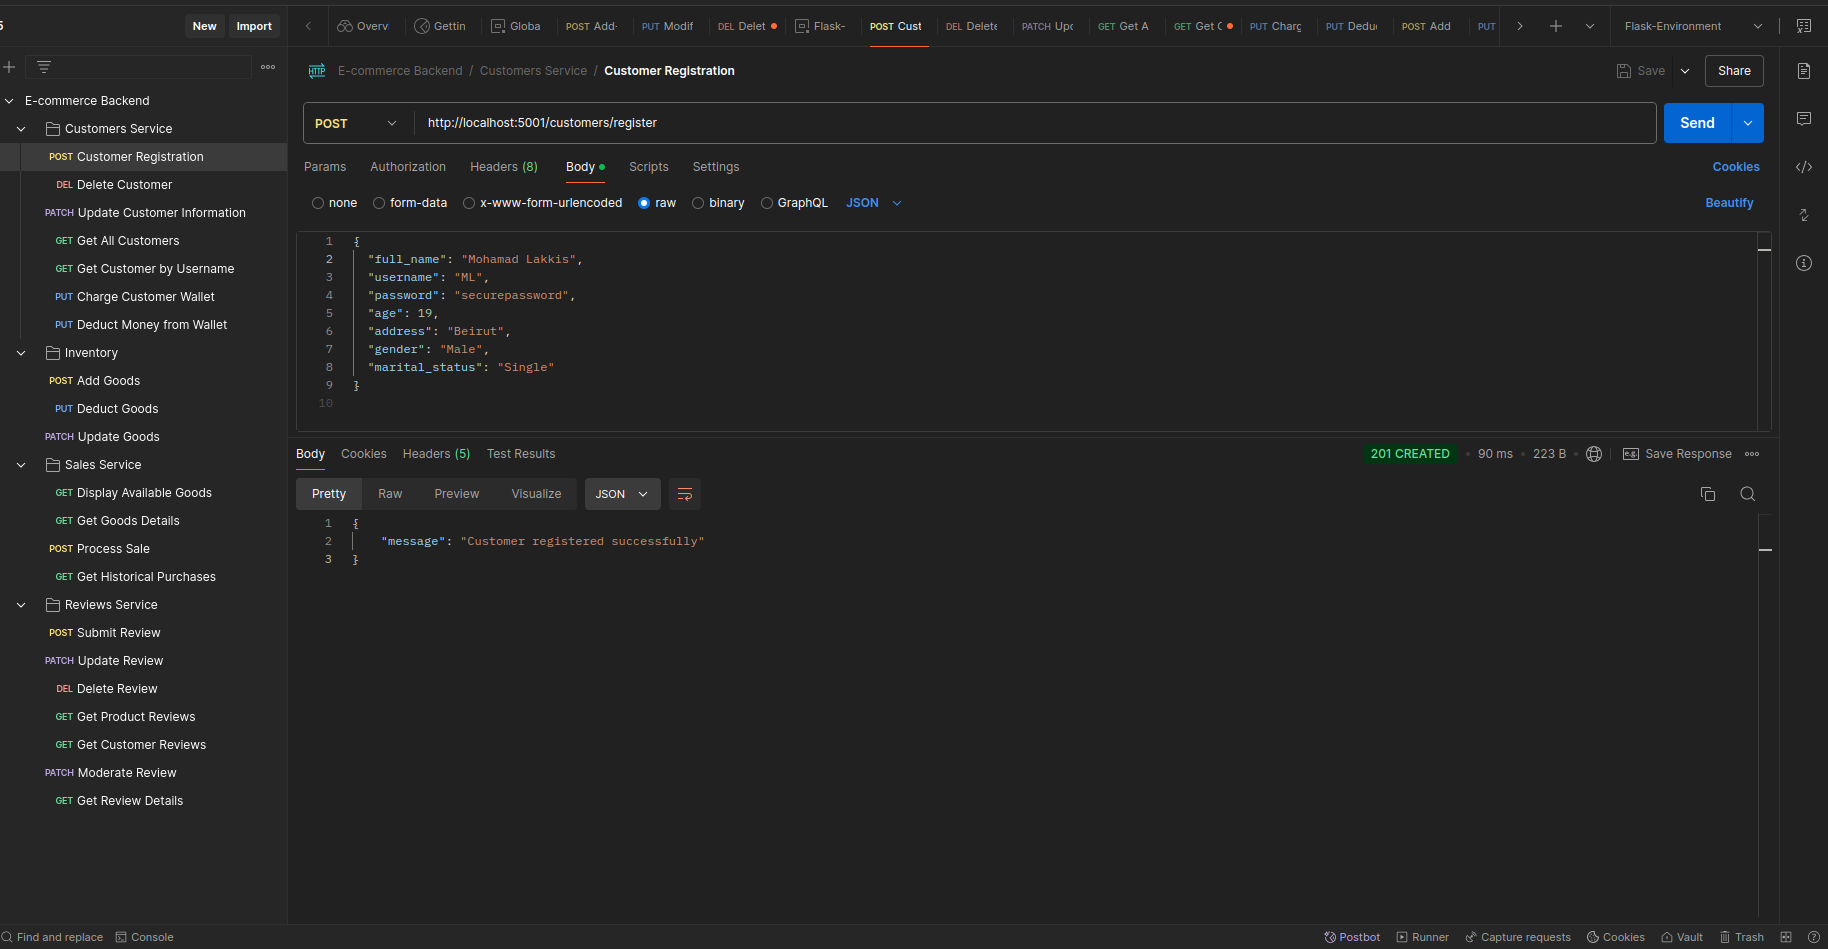
\includegraphics[width=0.6\textwidth]{images/1.png}
  \caption{Customer registration}
\end{figure}
\begin{figure}[H]
  \centering
  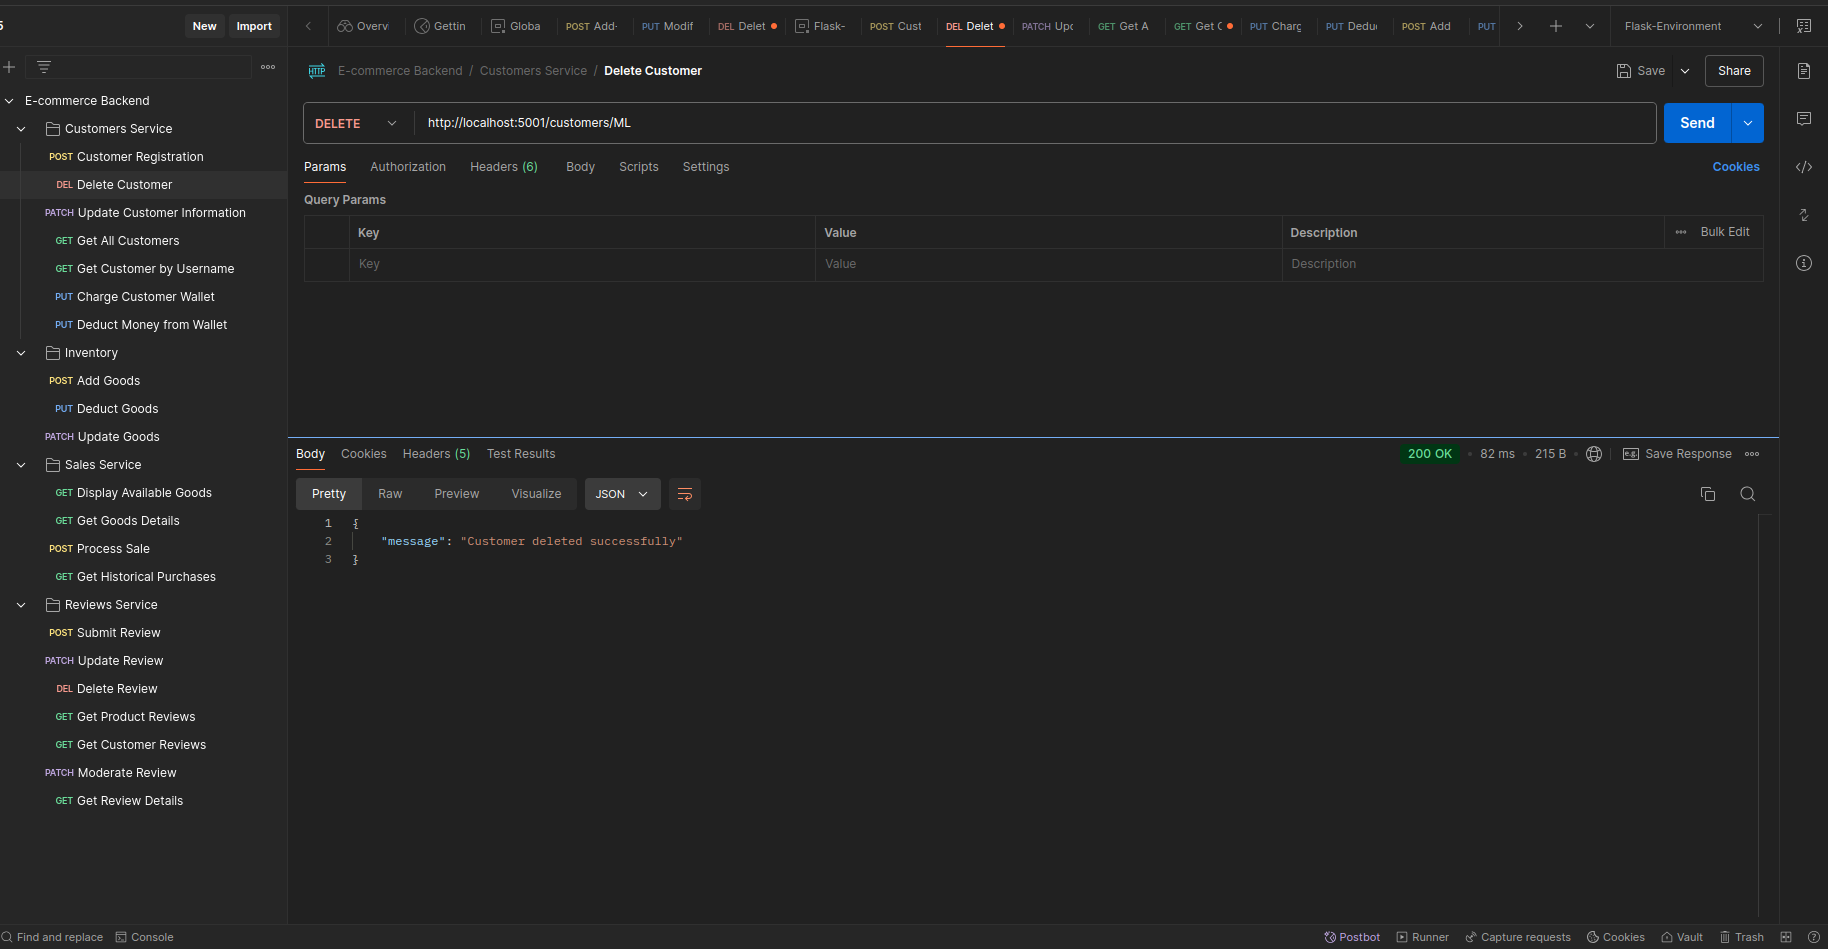
\includegraphics[width=0.6\textwidth]{images/2.png}
  \caption{Delete customer}
\end{figure}
\begin{figure}[H]
  \centering
  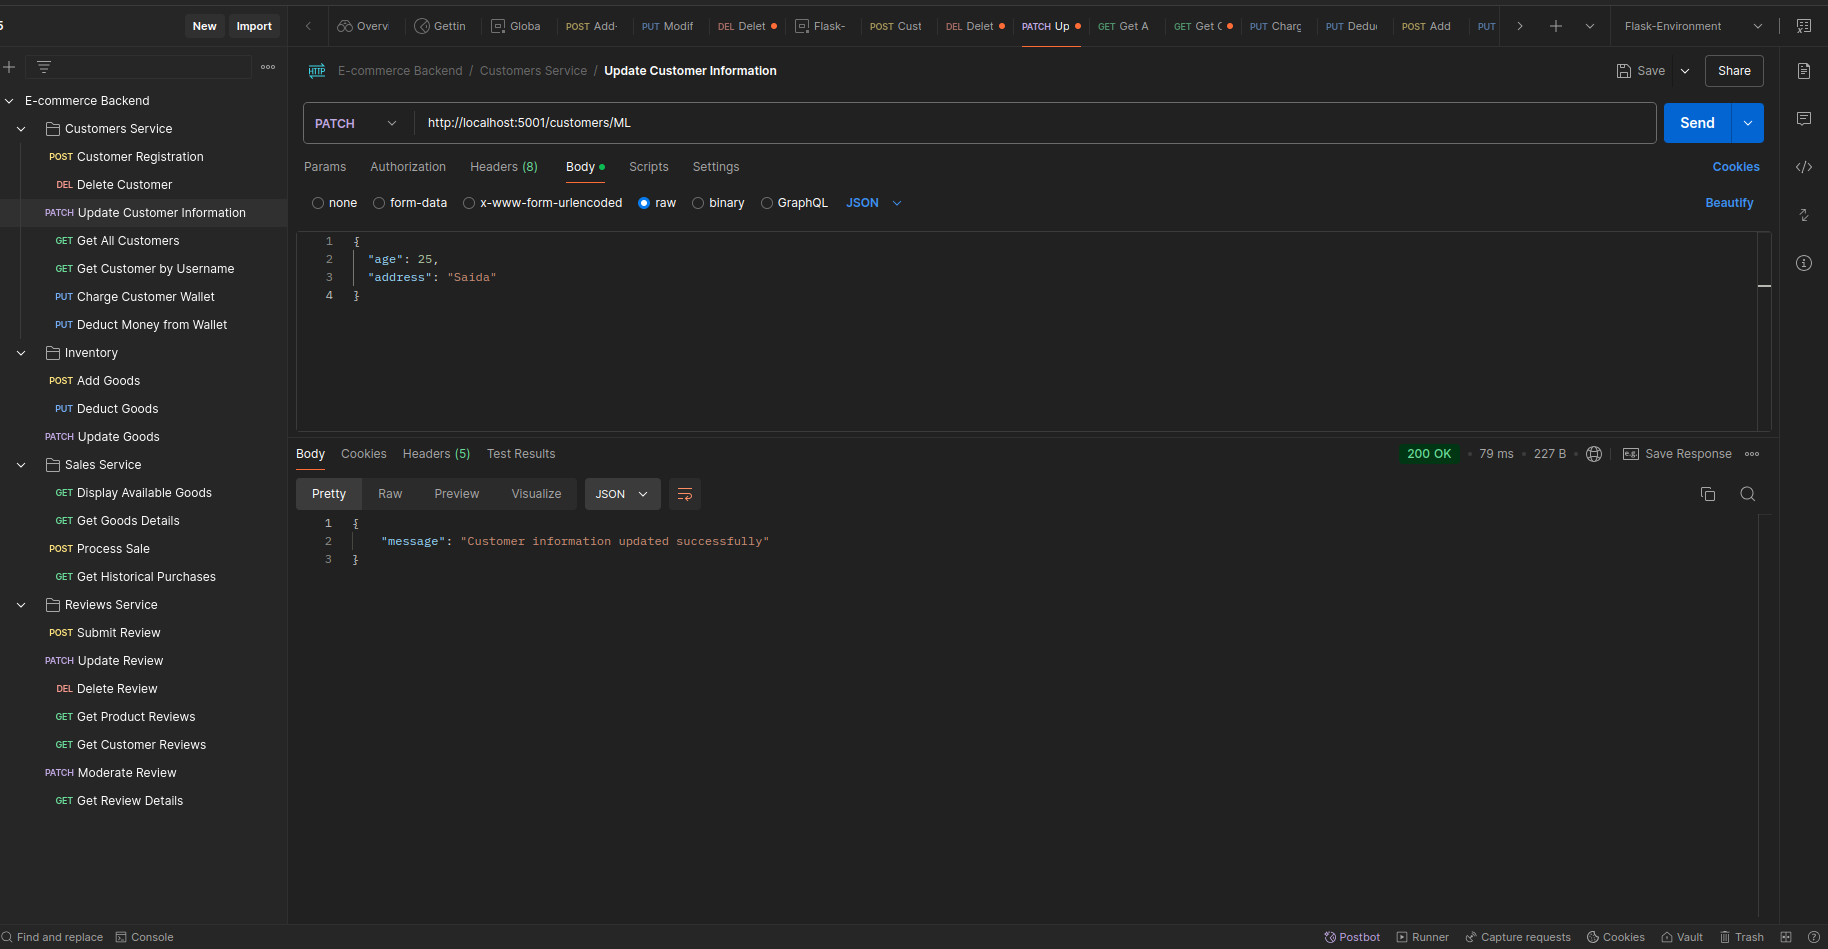
\includegraphics[width=0.6\textwidth]{images/3.png}
  \caption{Update customer information}
\end{figure}
\begin{figure}[H]
  \centering
  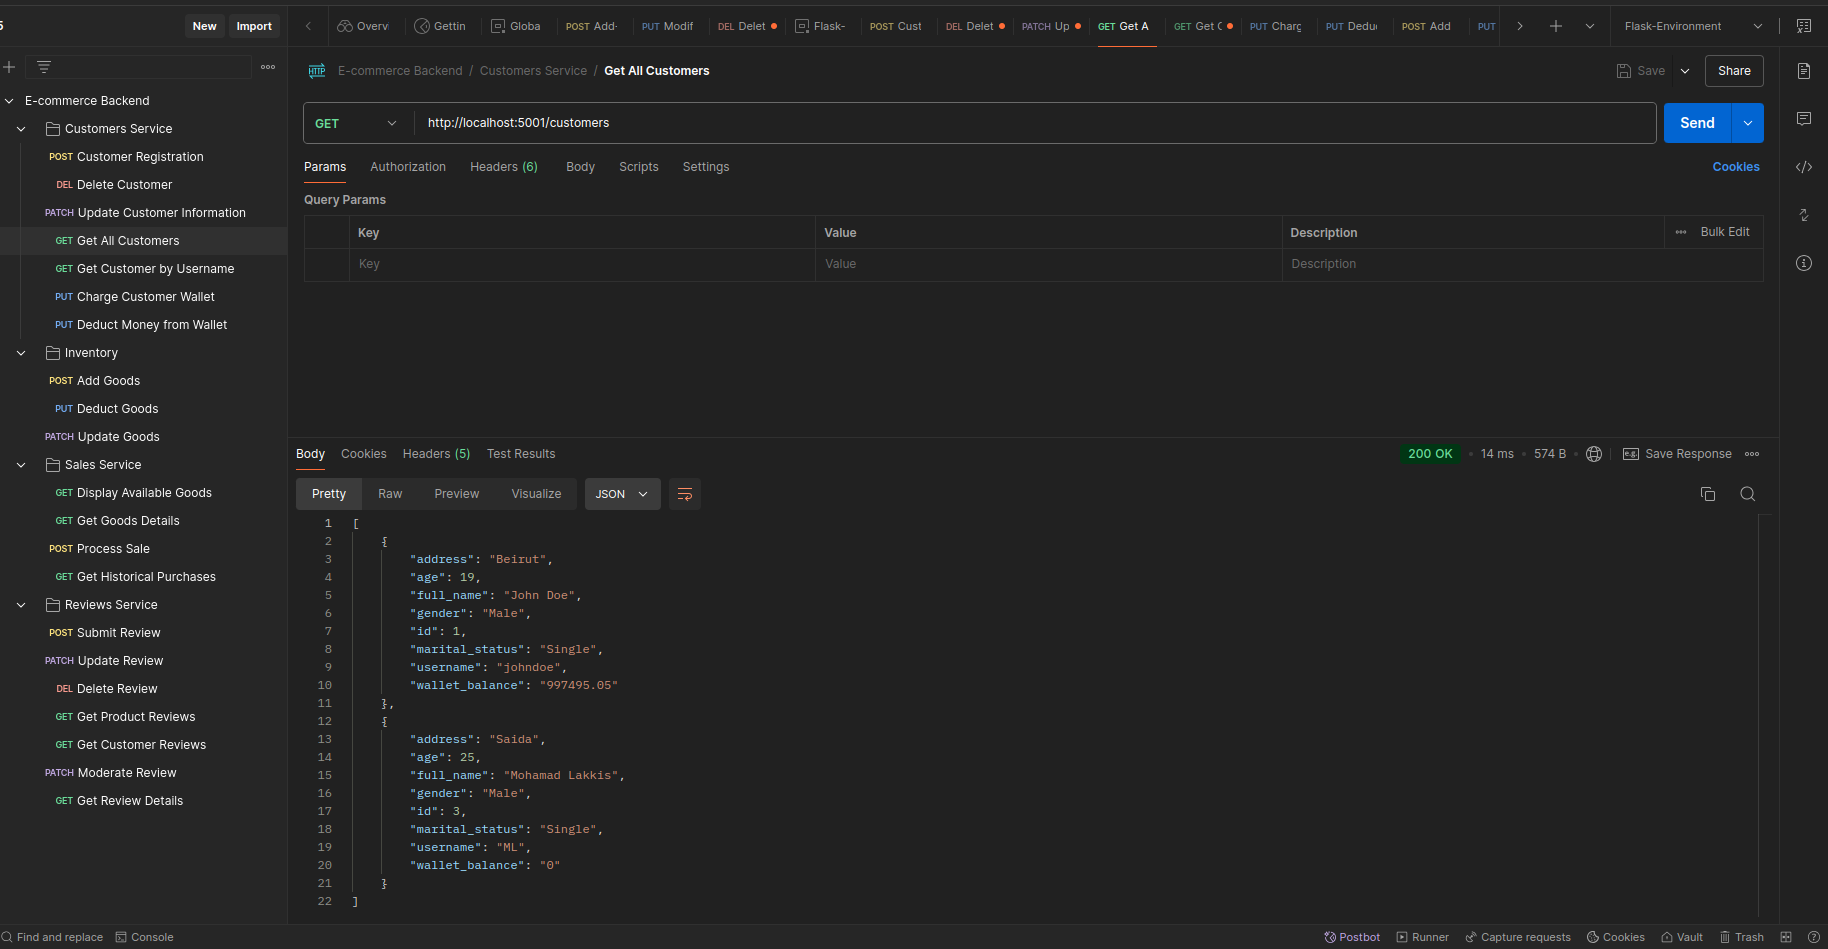
\includegraphics[width=0.6\textwidth]{images/4.png}
  \caption{Get all customers}
\end{figure}
\begin{figure}[H]
  \centering
  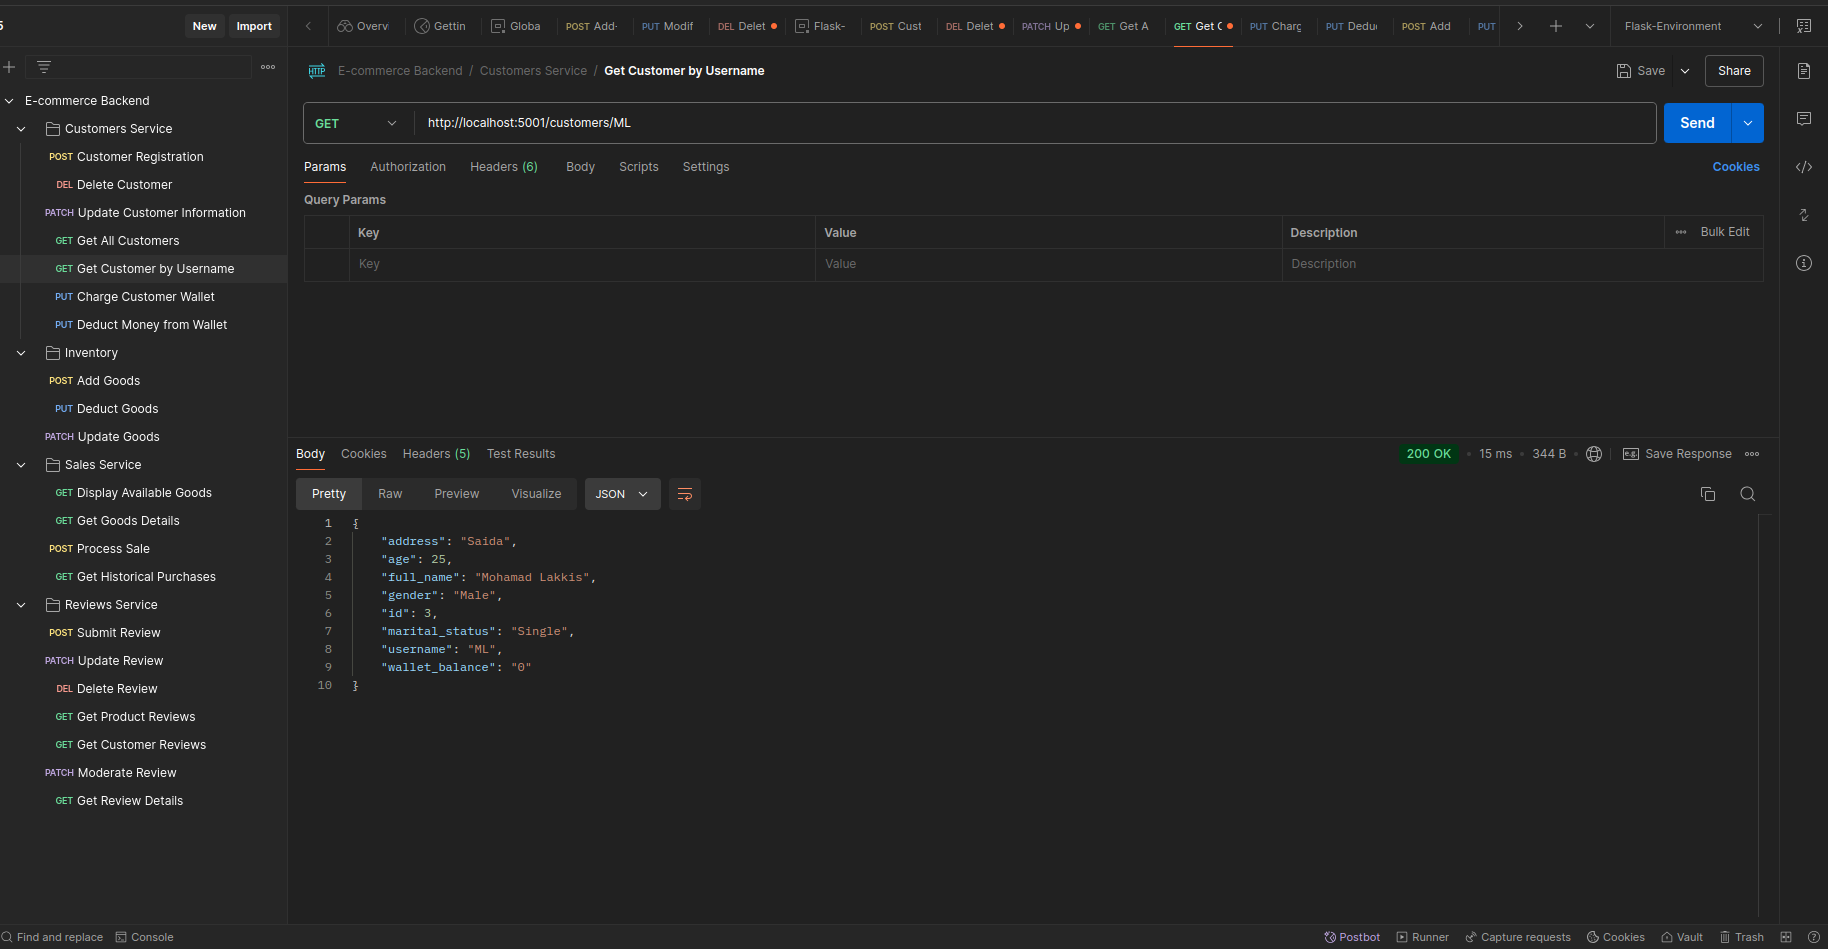
\includegraphics[width=0.6\textwidth]{images/5.png}
  \caption{Get customer per username}
\end{figure}
\begin{figure}[H]
  \centering
  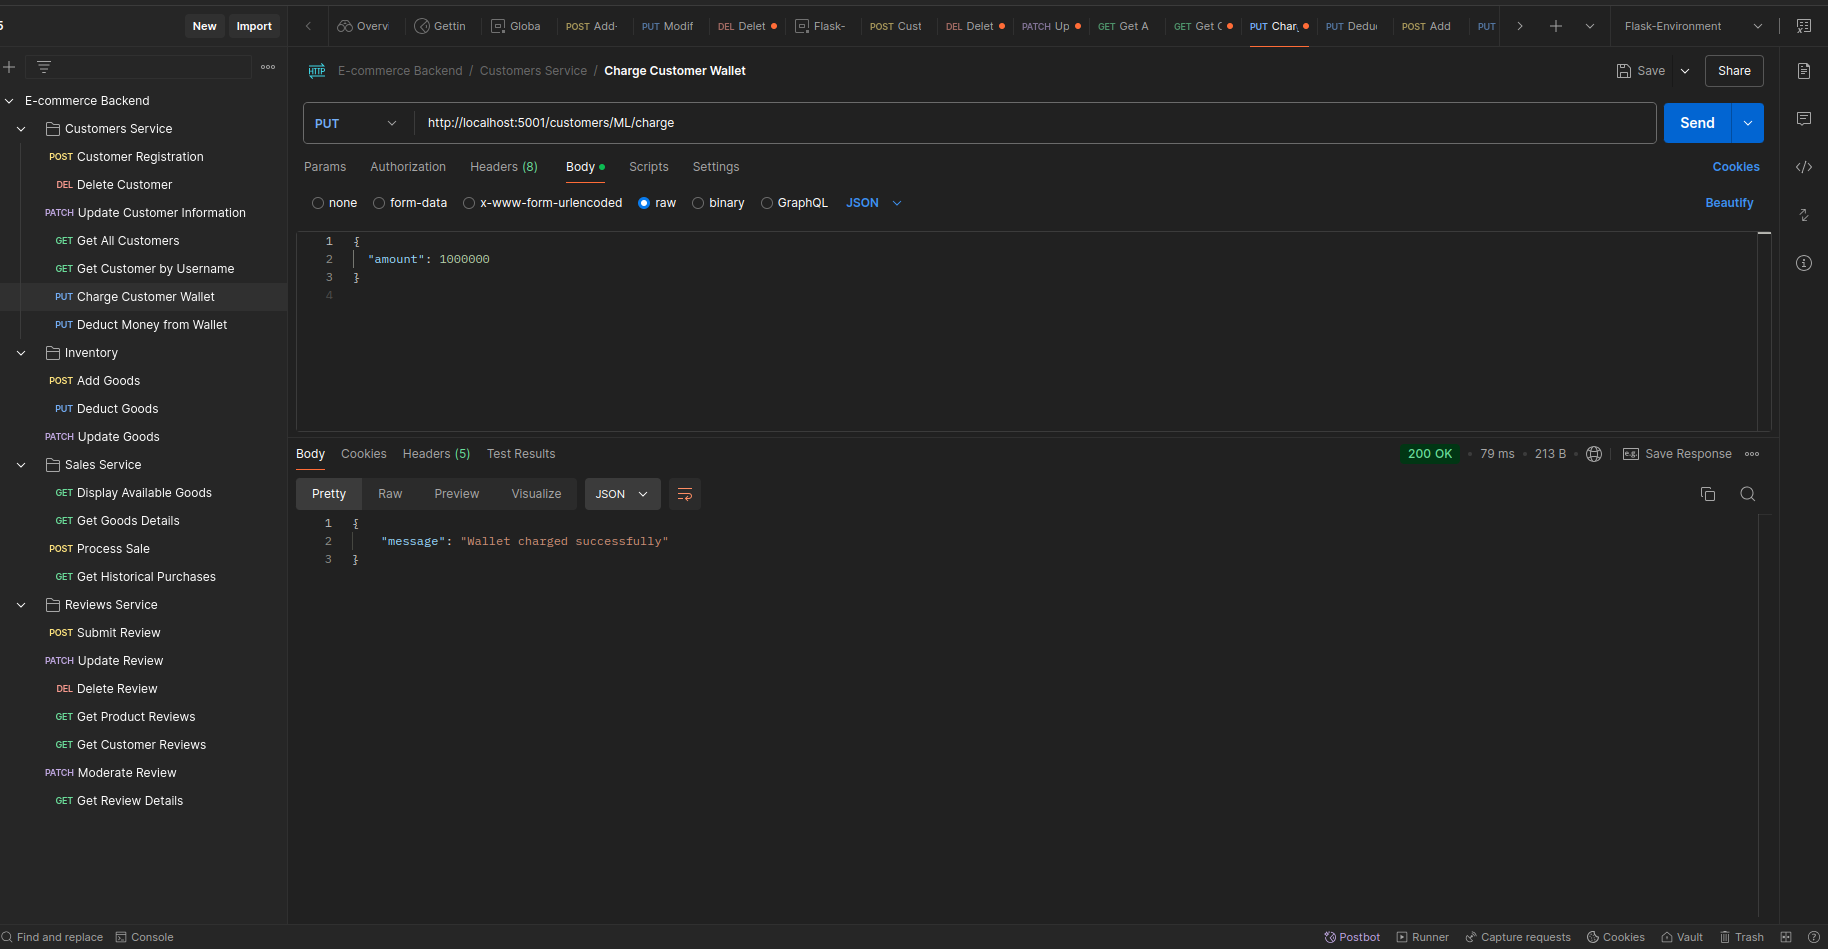
\includegraphics[width=0.6\textwidth]{images/6.png}
  \caption{Charge customer wallet in dollars}
\end{figure}
\begin{figure}[H]
  \centering
  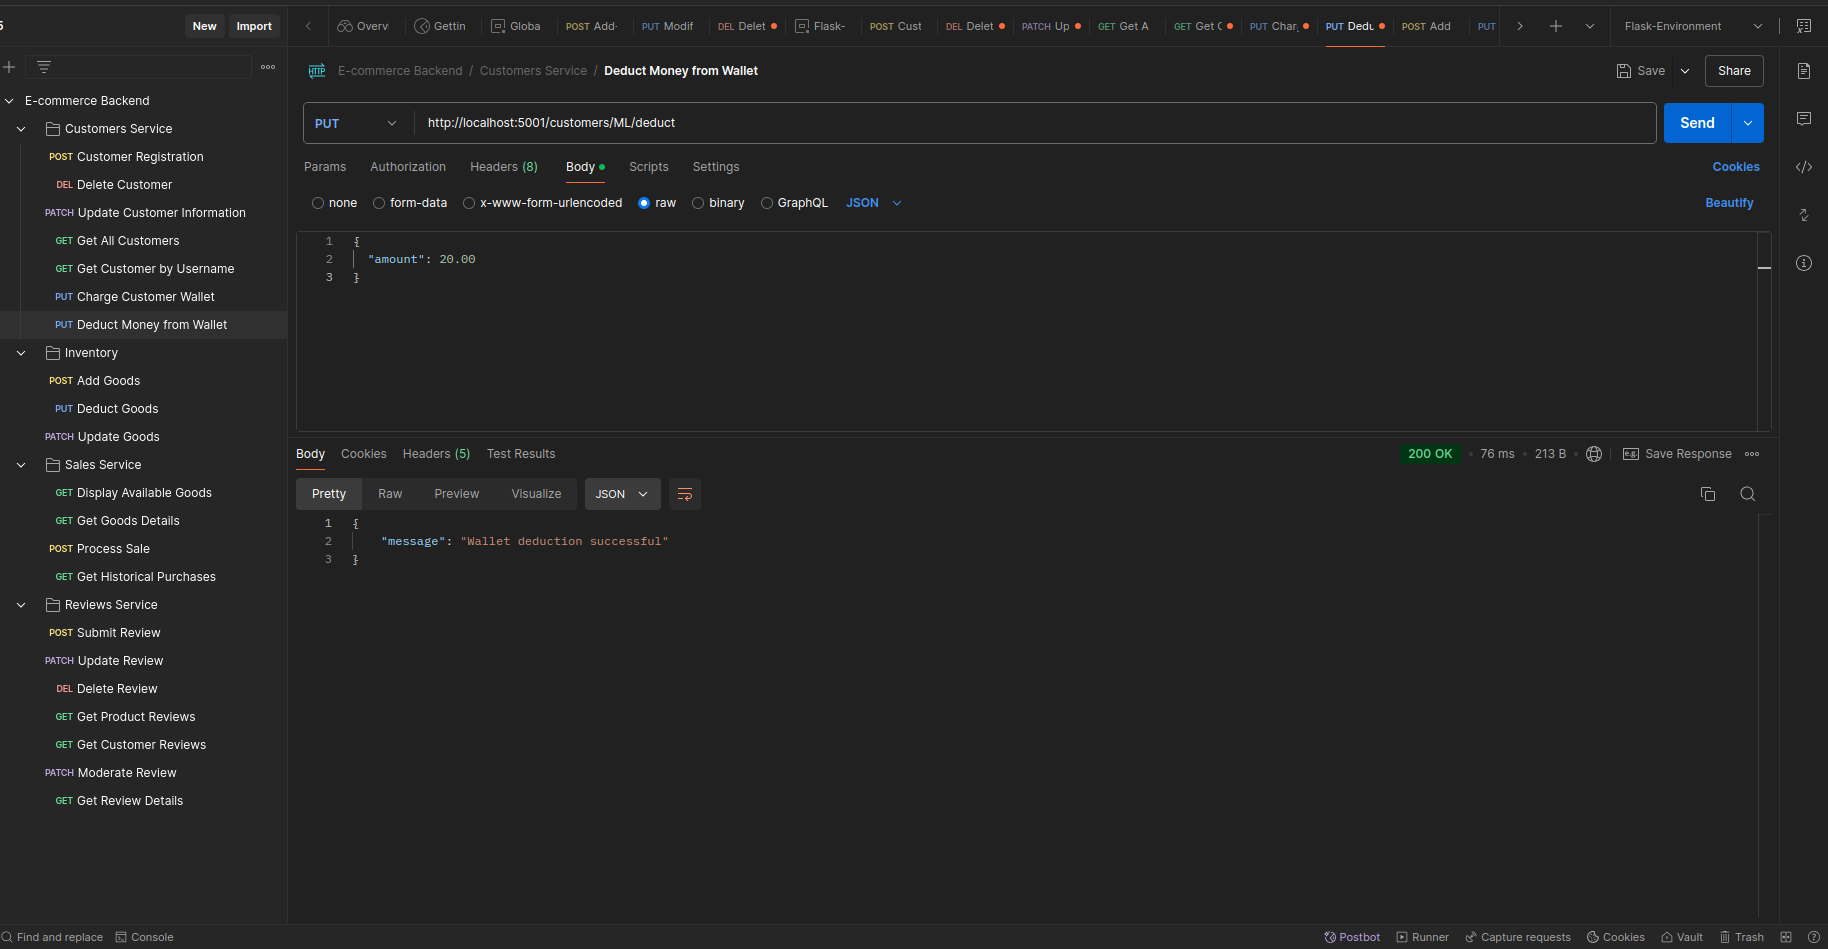
\includegraphics[width=0.6\textwidth]{images/7.png}
  \caption{Deduct wallet funds}
\end{figure}
\subsection{Inventory Service}
\subsubsection{Description}
Handles inventory management, including adding, updating, and removing goods.

\subsubsection{APIs}
\begin{longtable}{|p{4cm}|p{2cm}|p{7cm}|}
\hline
\textbf{API} & \textbf{Method} & \textbf{Description} \\
\hline
Add Goods & POST & Adds a new product to the inventory. \\
\hline
Deduct Goods & PUT & Removes items from stock. \\
\hline
Update Goods & PATCH & Updates product details. \\
\hline
\end{longtable}

\subsubsection{Running Port}
Port: \textbf{5002}

\subsubsection{Database Structure}
\begin{longtable}{|p{3cm}|p{3cm}|p{8cm}|}
\hline
\textbf{Field} & \textbf{Type} & \textbf{Description} \\
\hline
id & SERIAL (PK) & Unique identifier for the product. \\
\hline
name & VARCHAR(100) & Name of the product. \\
\hline
category & VARCHAR(50) & Category of the product (e.g., food). \\
\hline
price & NUMERIC & Price per item. \\
\hline
description & TEXT & Detailed description of the product. \\
\hline
count & INTEGER & Available stock count. \\
\hline
\end{longtable}
\subsubsection{Postman Testing}
\begin{figure}[H]
  \centering
  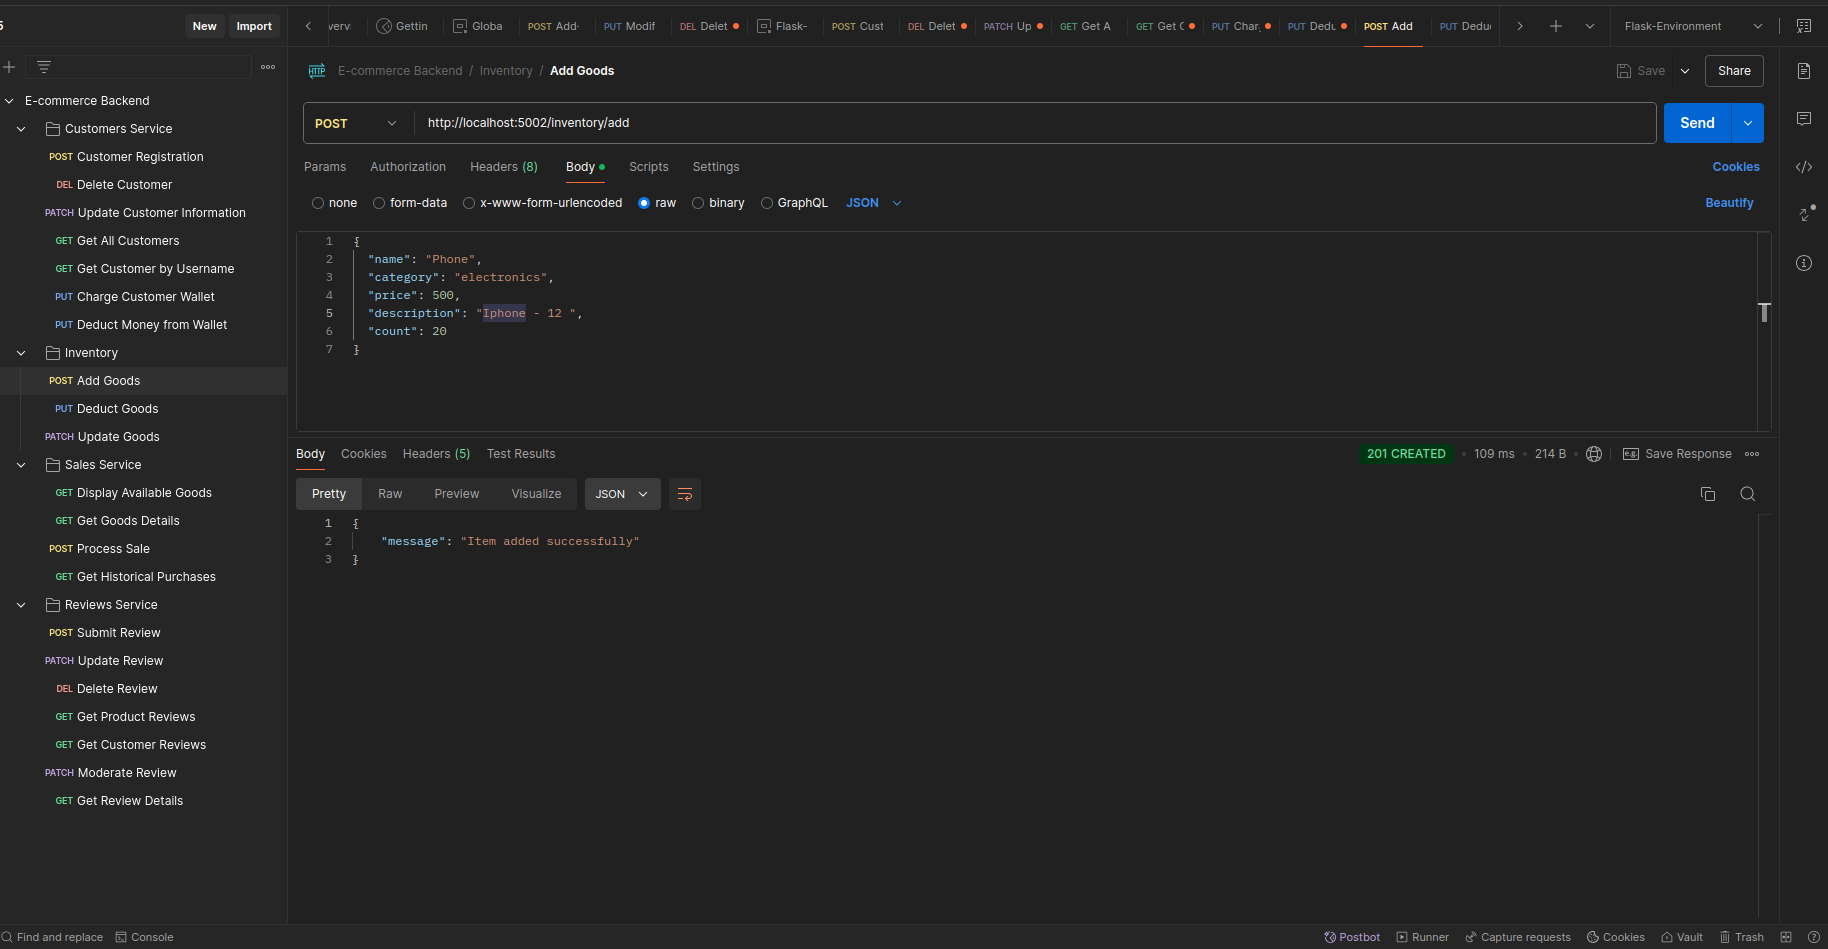
\includegraphics[width=0.6\textwidth]{images/8.png}
  \caption{Add goods}
\end{figure}
\begin{figure}[H]
  \centering
  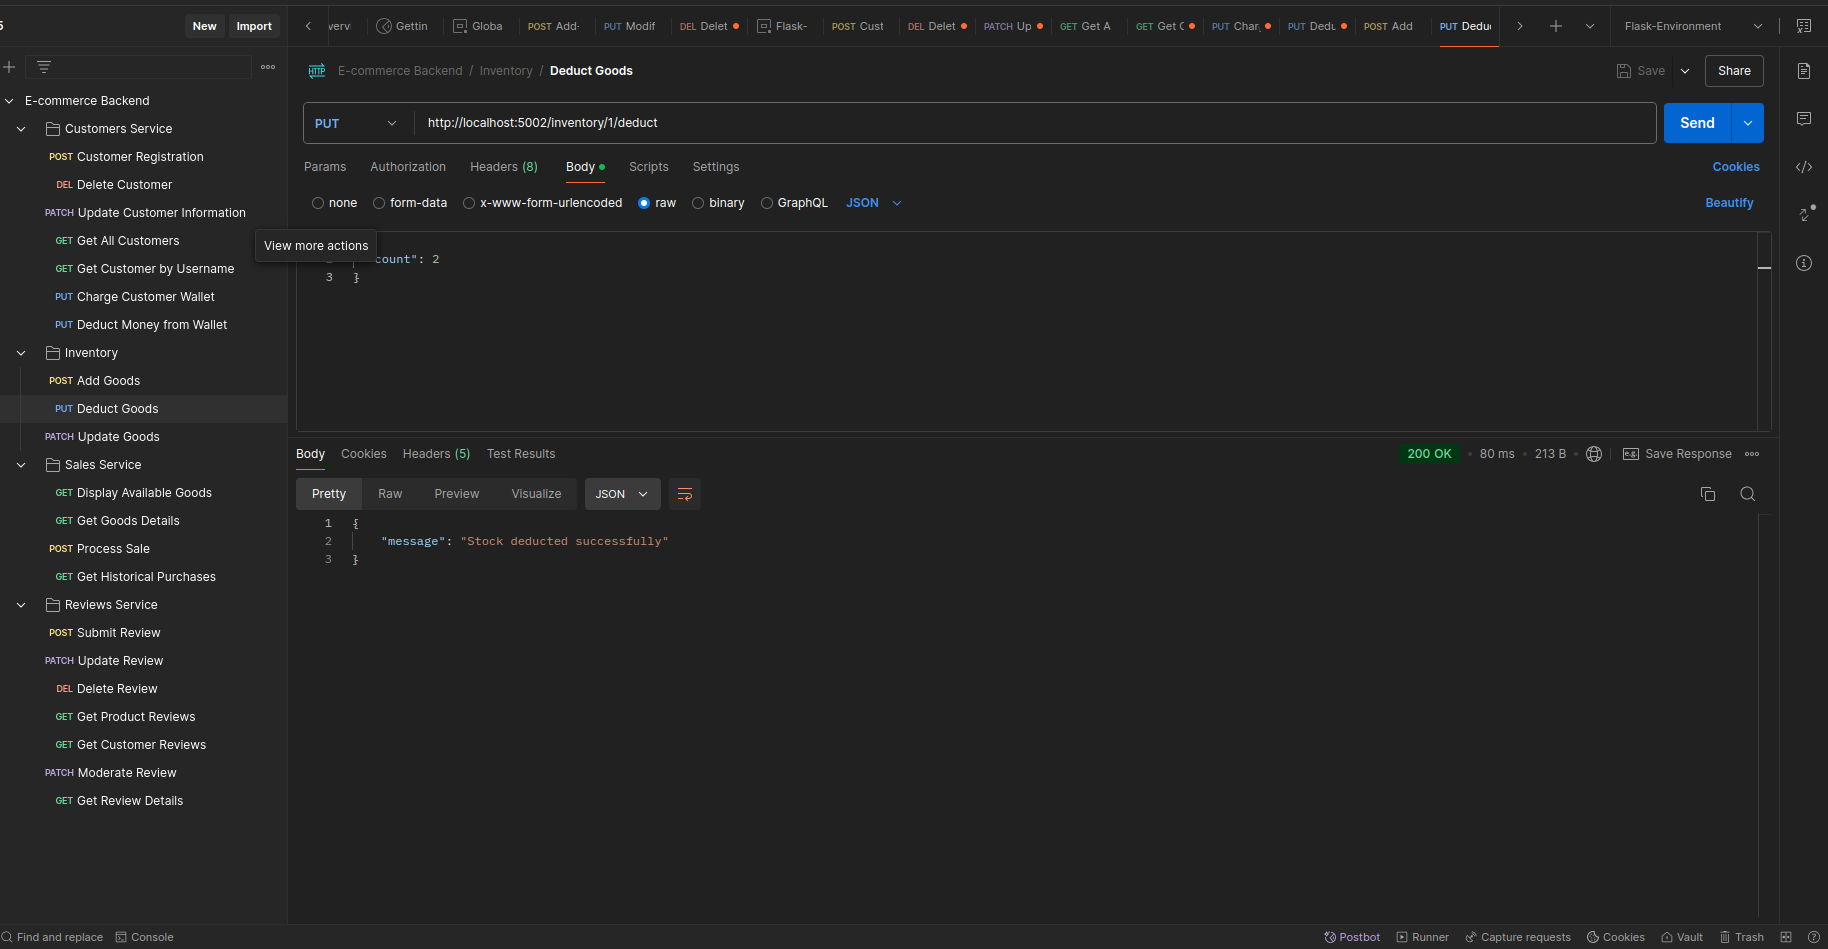
\includegraphics[width=0.6\textwidth]{images/9.png}
  \caption{Deduct goods}
\end{figure}
\begin{figure}[H]
  \centering
  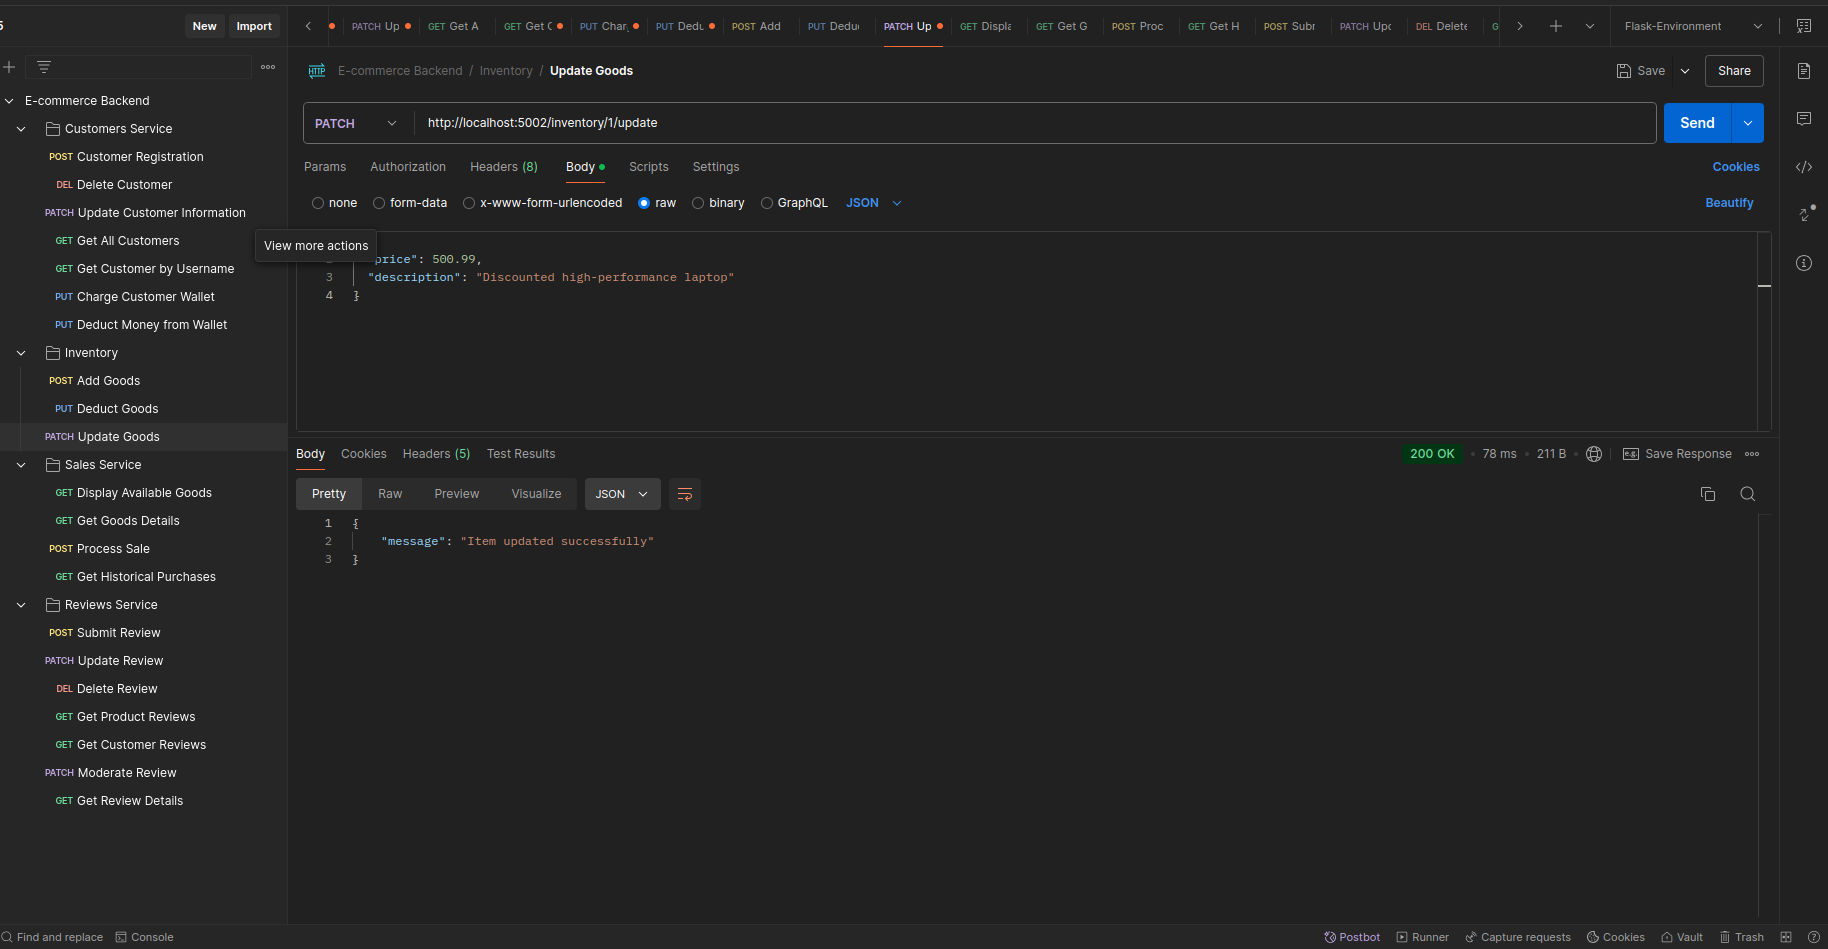
\includegraphics[width=0.6\textwidth]{images/10.png}
  \caption{Update goods}
\end{figure}



\subsection{Sales Service}
\subsubsection{Description}
Manages the sale of goods, including processing purchases and tracking historical sales.

\subsubsection{APIs}
\begin{longtable}{|p{4cm}|p{2cm}|p{7cm}|}
\hline
\textbf{API} & \textbf{Method} & \textbf{Description} \\
\hline
Display Goods & GET & Lists all available goods with prices. \\
\hline
Get Goods Details & GET & Retrieves detailed information about a product. \\
\hline
Process Sale & POST & Processes a sale by deducting stock and funds. \\
\hline
Get Purchase History & GET & Retrieves historical purchases for a customer. \\
\hline
\end{longtable}

\subsubsection{Running Port}
Port: \textbf{5003}

\subsubsection{Database Structure}
\begin{longtable}{|p{3cm}|p{3cm}|p{8cm}|}
\hline
\textbf{Field} & \textbf{Type} & \textbf{Description} \\
\hline
id & SERIAL (PK) & Unique identifier for the sale. \\
\hline
customer\_id & INTEGER (FK) & References the customer making the purchase. \\
\hline
good\_id & INTEGER (FK) & References the product being purchased. \\
\hline
quantity & INTEGER & Number of items purchased. \\
\hline
total\_price & NUMERIC & Total price of the purchase. \\
\hline
sale\_date & TIMESTAMP & Date and time of the purchase. \\
\hline
\end{longtable}
\subsubsection{Postman Testing}
\begin{figure}[H]
  \centering
  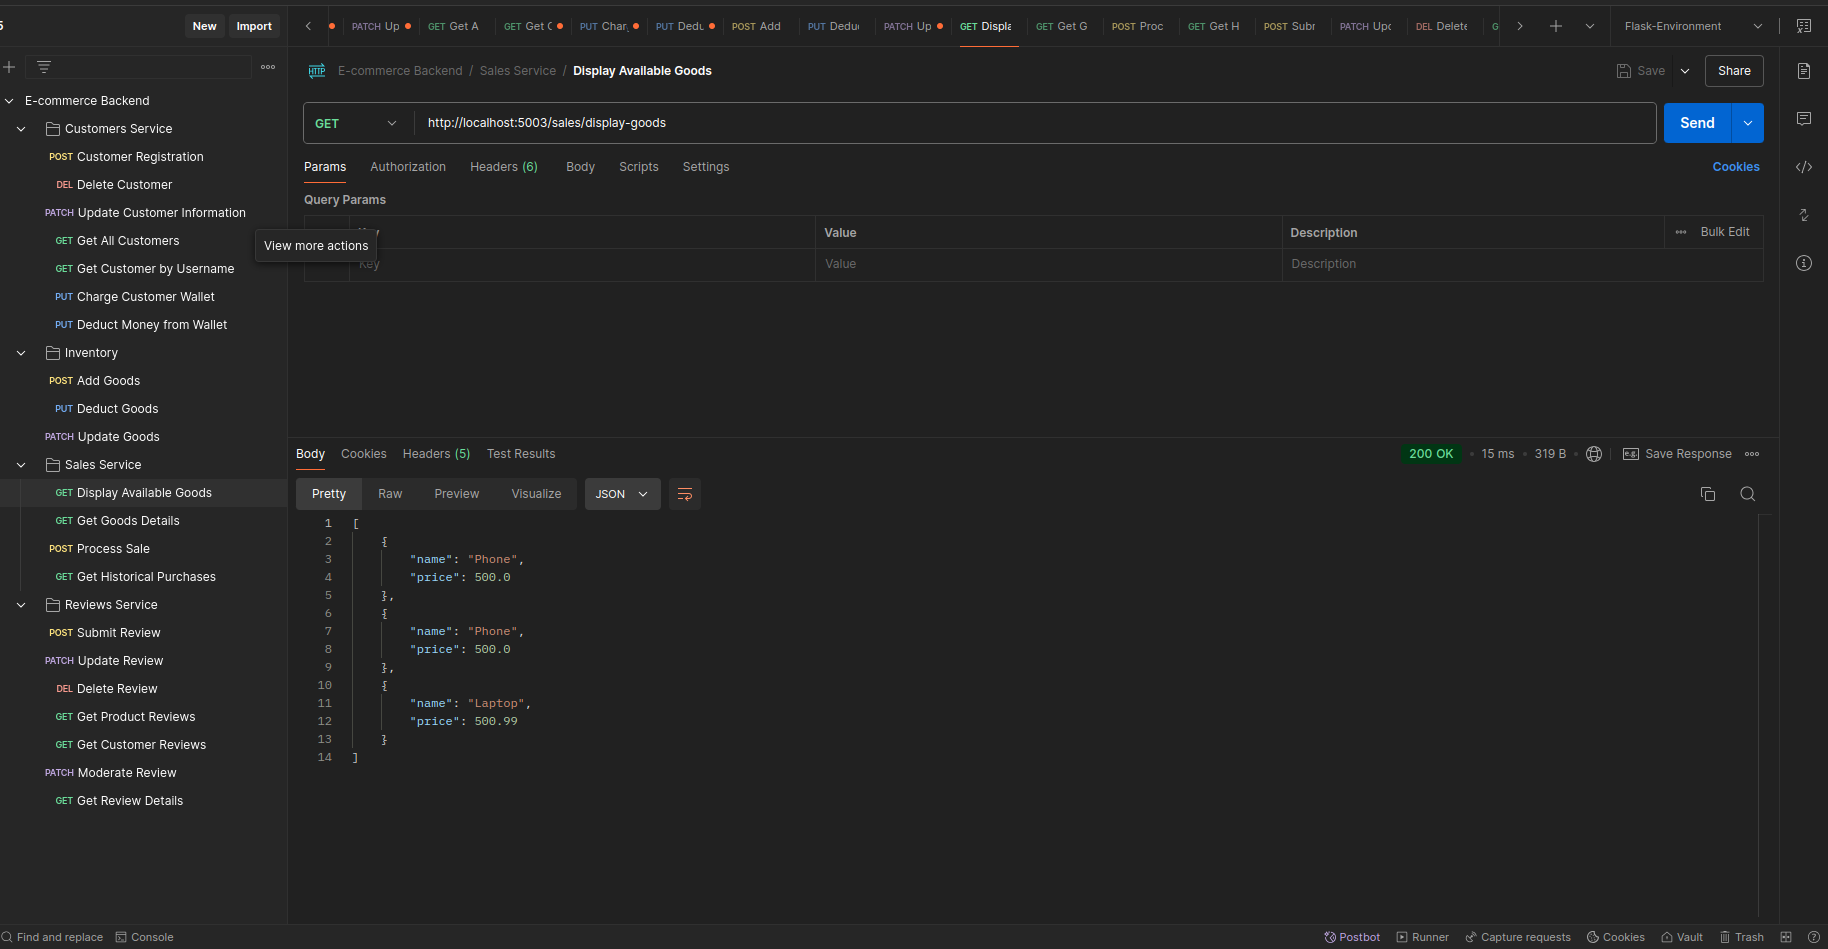
\includegraphics[width=0.6\textwidth]{images/11.png}
  \caption{Display goods}
\end{figure}
\begin{figure}[H]
  \centering
  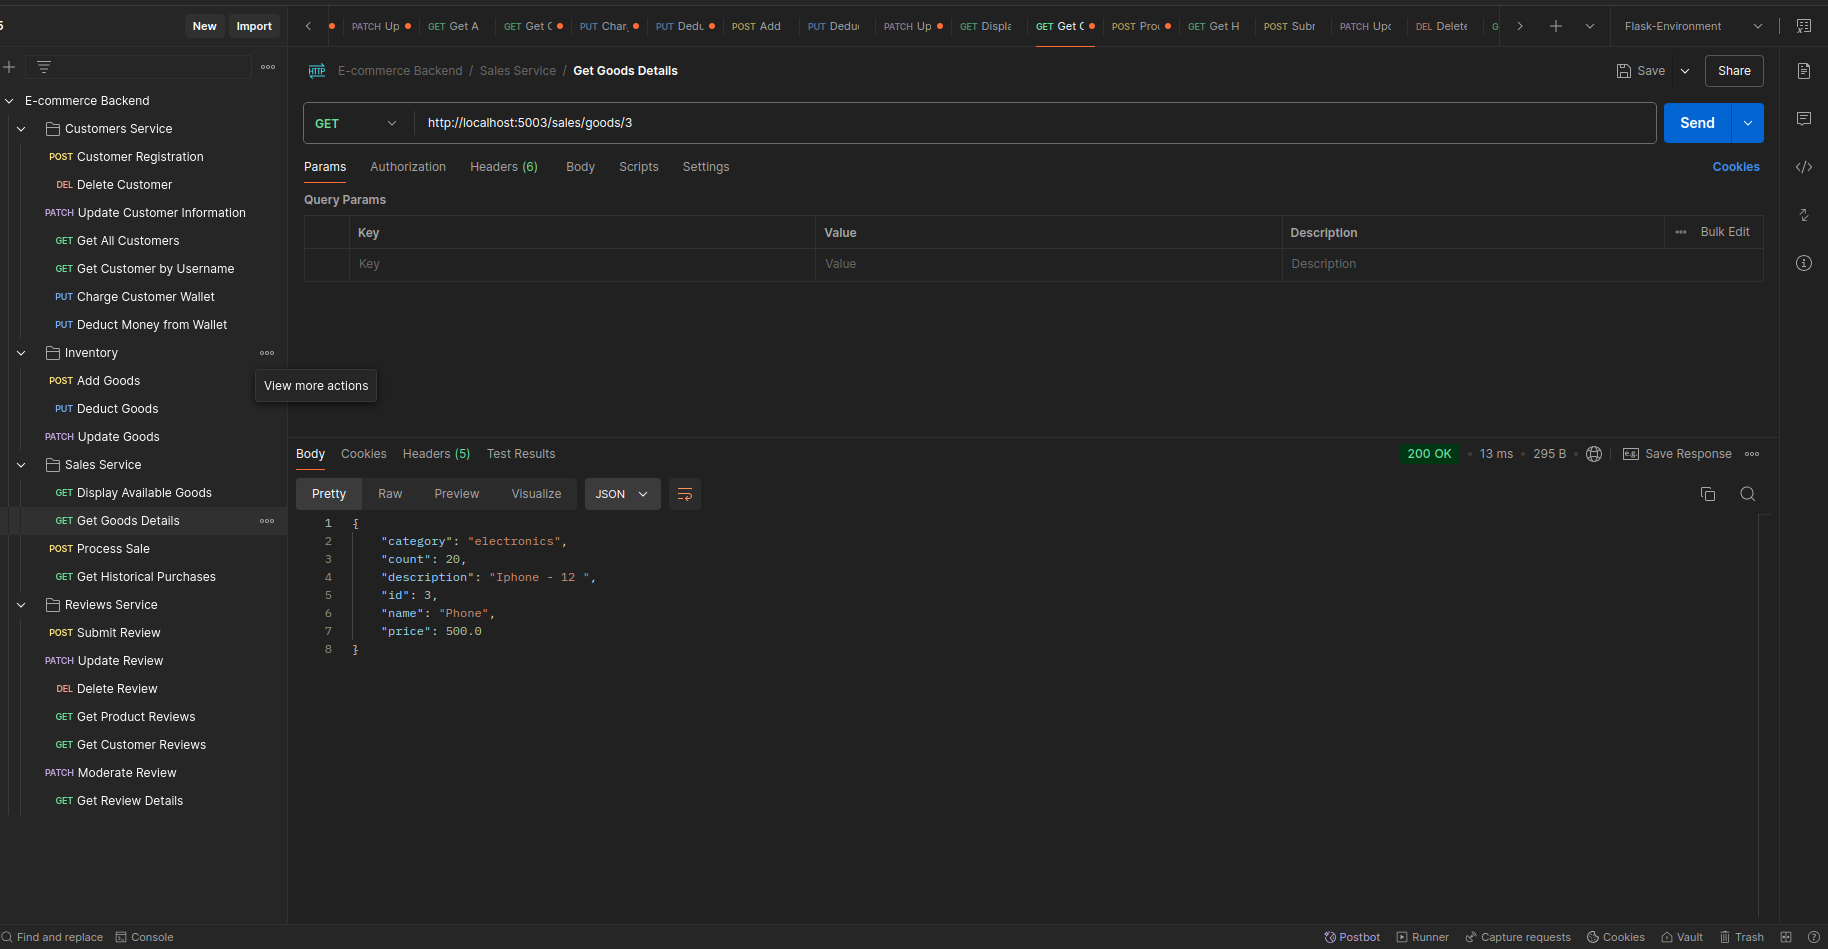
\includegraphics[width=0.6\textwidth]{images/12.png}
  \caption{Get goods details}
\end{figure}
\begin{figure}[H]
  \centering
  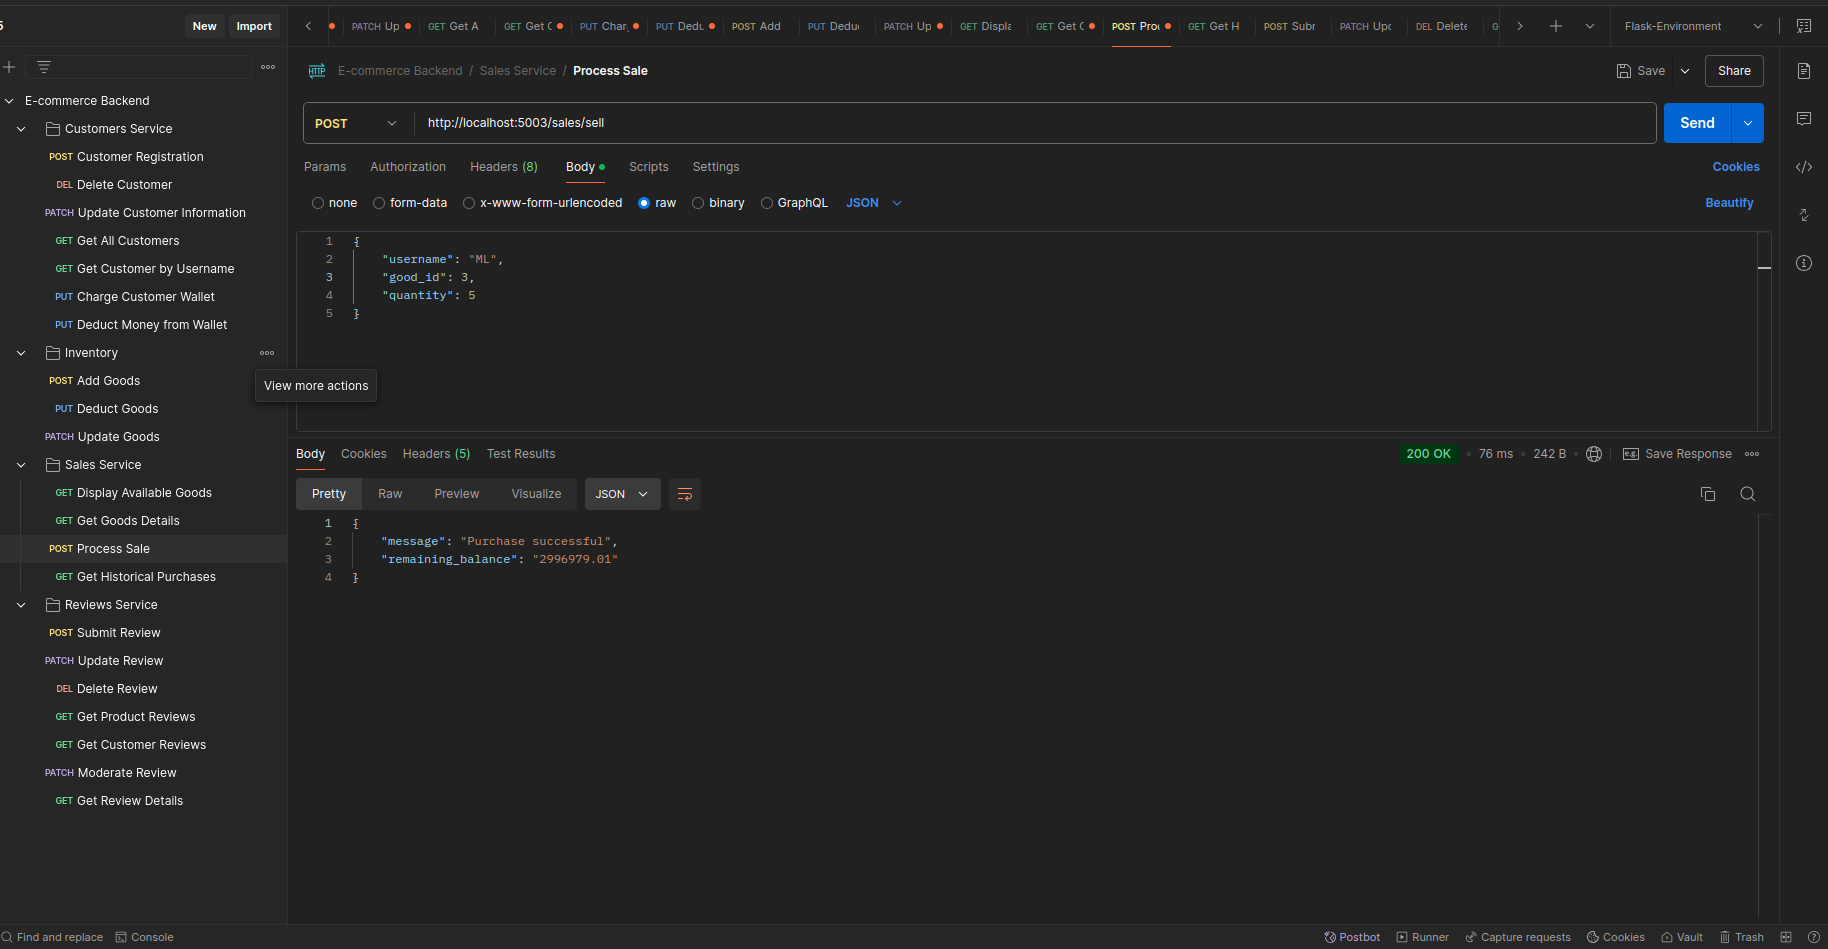
\includegraphics[width=0.6\textwidth]{images/13.png}
  \caption{Process sale}
\end{figure}
\begin{figure}[H]
  \centering
  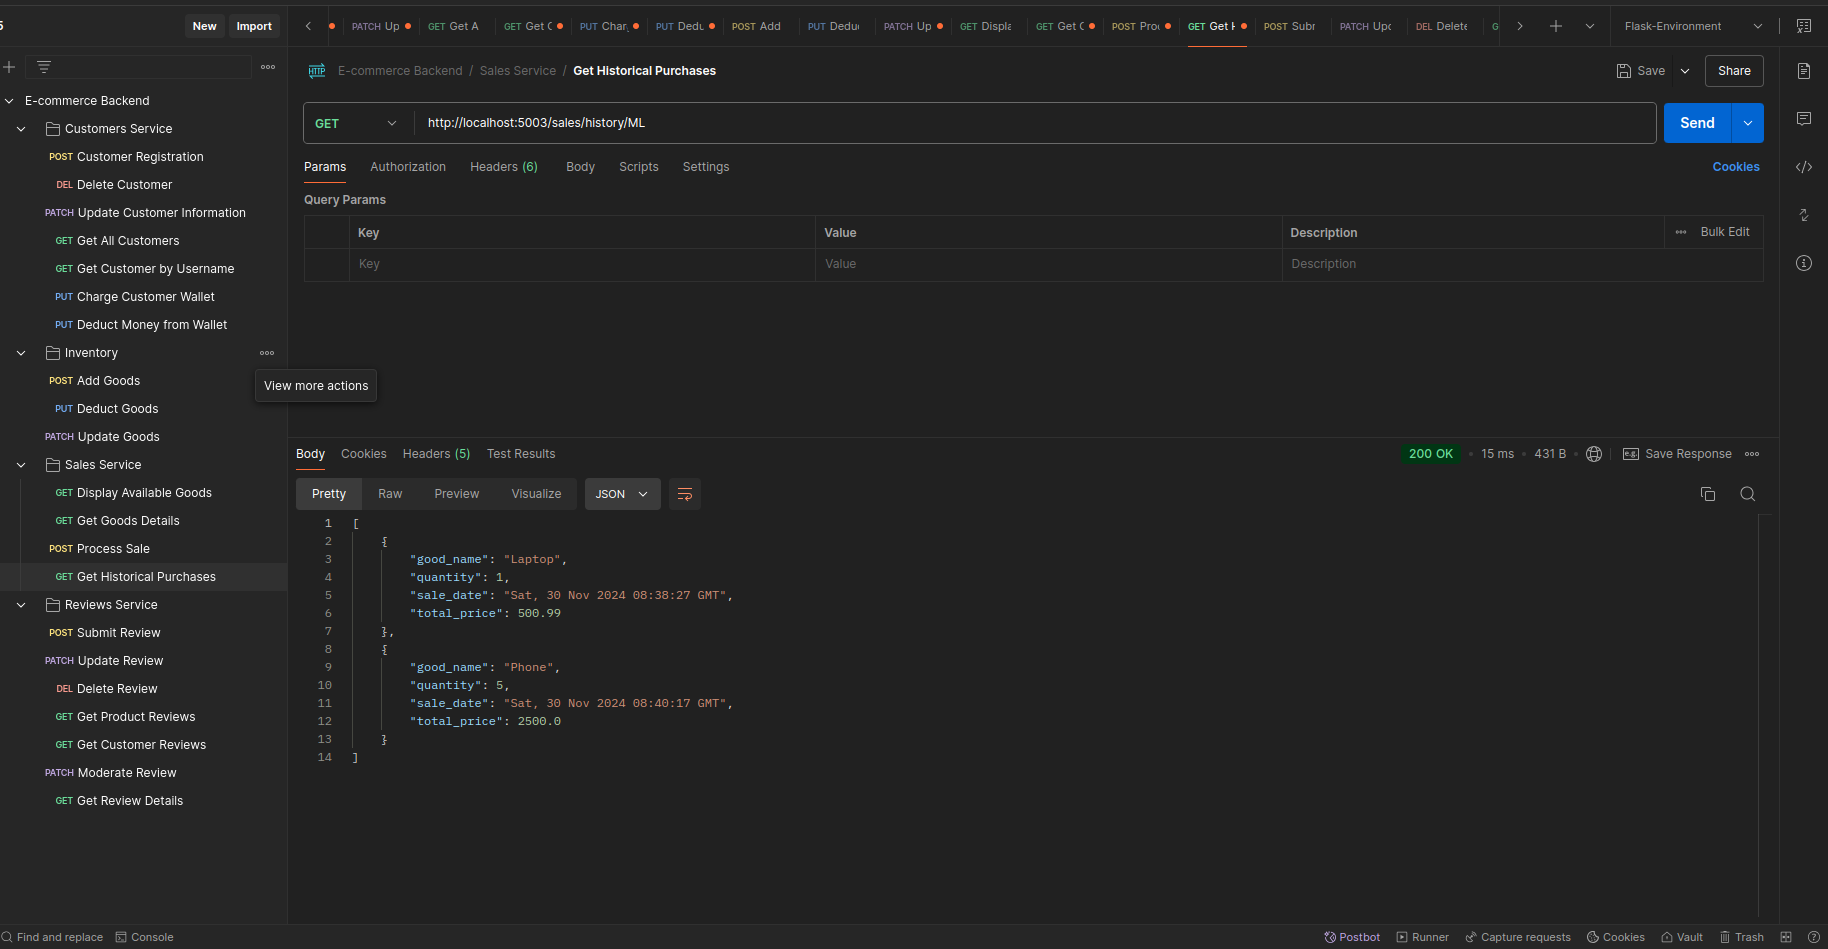
\includegraphics[width=0.6\textwidth]{images/14.png}
  \caption{Get purchase history}
\end{figure}


\subsection{Reviews Service}
\subsubsection{Description}
Manages product reviews and ratings submitted by customers.

\subsubsection{APIs}
\begin{longtable}{|p{4cm}|p{2cm}|p{7cm}|}
\hline
\textbf{API} & \textbf{Method} & \textbf{Description} \\
\hline
Submit Review & POST & Submits a review for a product. \\
\hline
Update Review & PATCH & Updates a specific review. \\
\hline
Delete Review & DELETE & Deletes a specific review. \\
\hline
Get Product Reviews & GET & Retrieves reviews for a specific product. \\
\hline
Get Customer Reviews & GET & Retrieves all reviews submitted by a customer. \\
\hline
Moderate Review & PATCH & Flags or approves a review. \\
\hline
Get Review Details & GET & Retrieves details of a specific review. \\
\hline
\end{longtable}

\subsubsection{Running Port}
Port: \textbf{5004}

\subsubsection{Database Structure}
\begin{longtable}{|p{3cm}|p{3cm}|p{8cm}|}
\hline
\textbf{Field} & \textbf{Type} & \textbf{Description} \\
\hline
id & SERIAL (PK) & Unique identifier for the review. \\
\hline
customer\_id & INTEGER (FK) & References the customer submitting the review. \\
\hline
product\_id & INTEGER (FK) & References the reviewed product. \\
\hline
rating & INTEGER & Rating given to the product (1-5). \\
\hline
comment & TEXT & Customer's feedback. \\
\hline
status & VARCHAR(20) & Status of the review (e.g., pending). \\
\hline
review\_date & TIMESTAMP & Date and time the review was submitted. \\
\hline
\end{longtable}
\subsubsection{Postman Testing}
\begin{figure}[H]
  \centering
  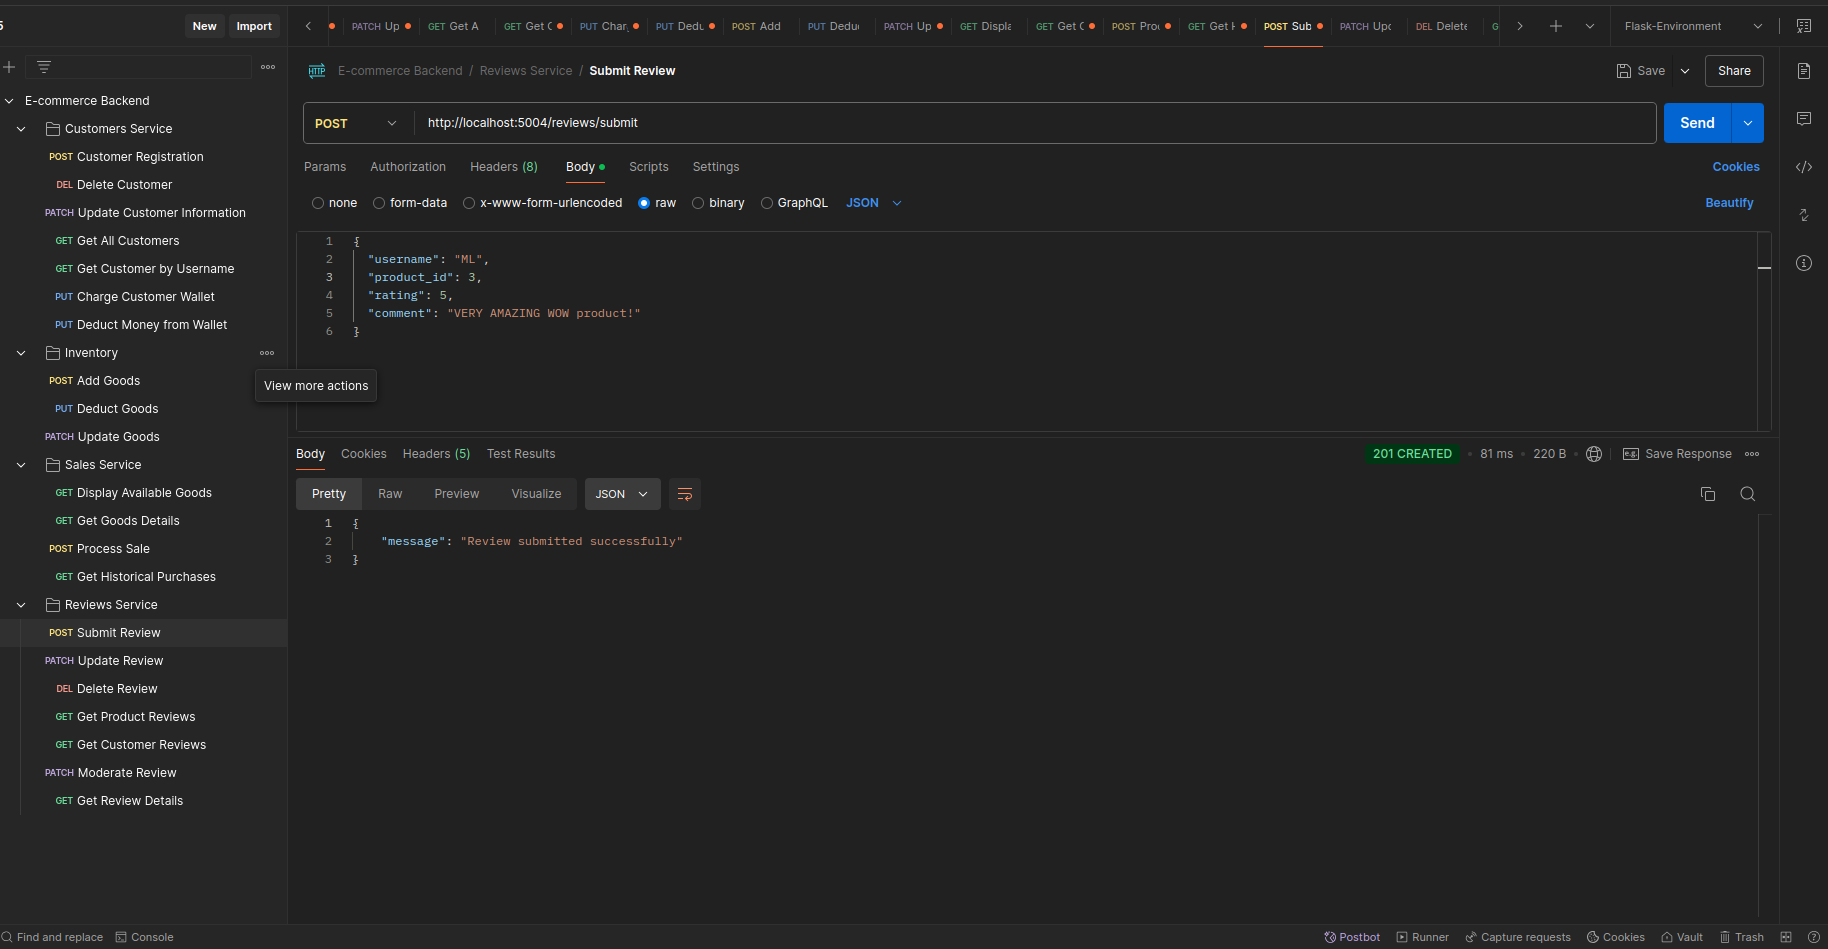
\includegraphics[width=0.6\textwidth]{images/15.png}
  \caption{Submit review}
\end{figure}
\begin{figure}[H]
  \centering
  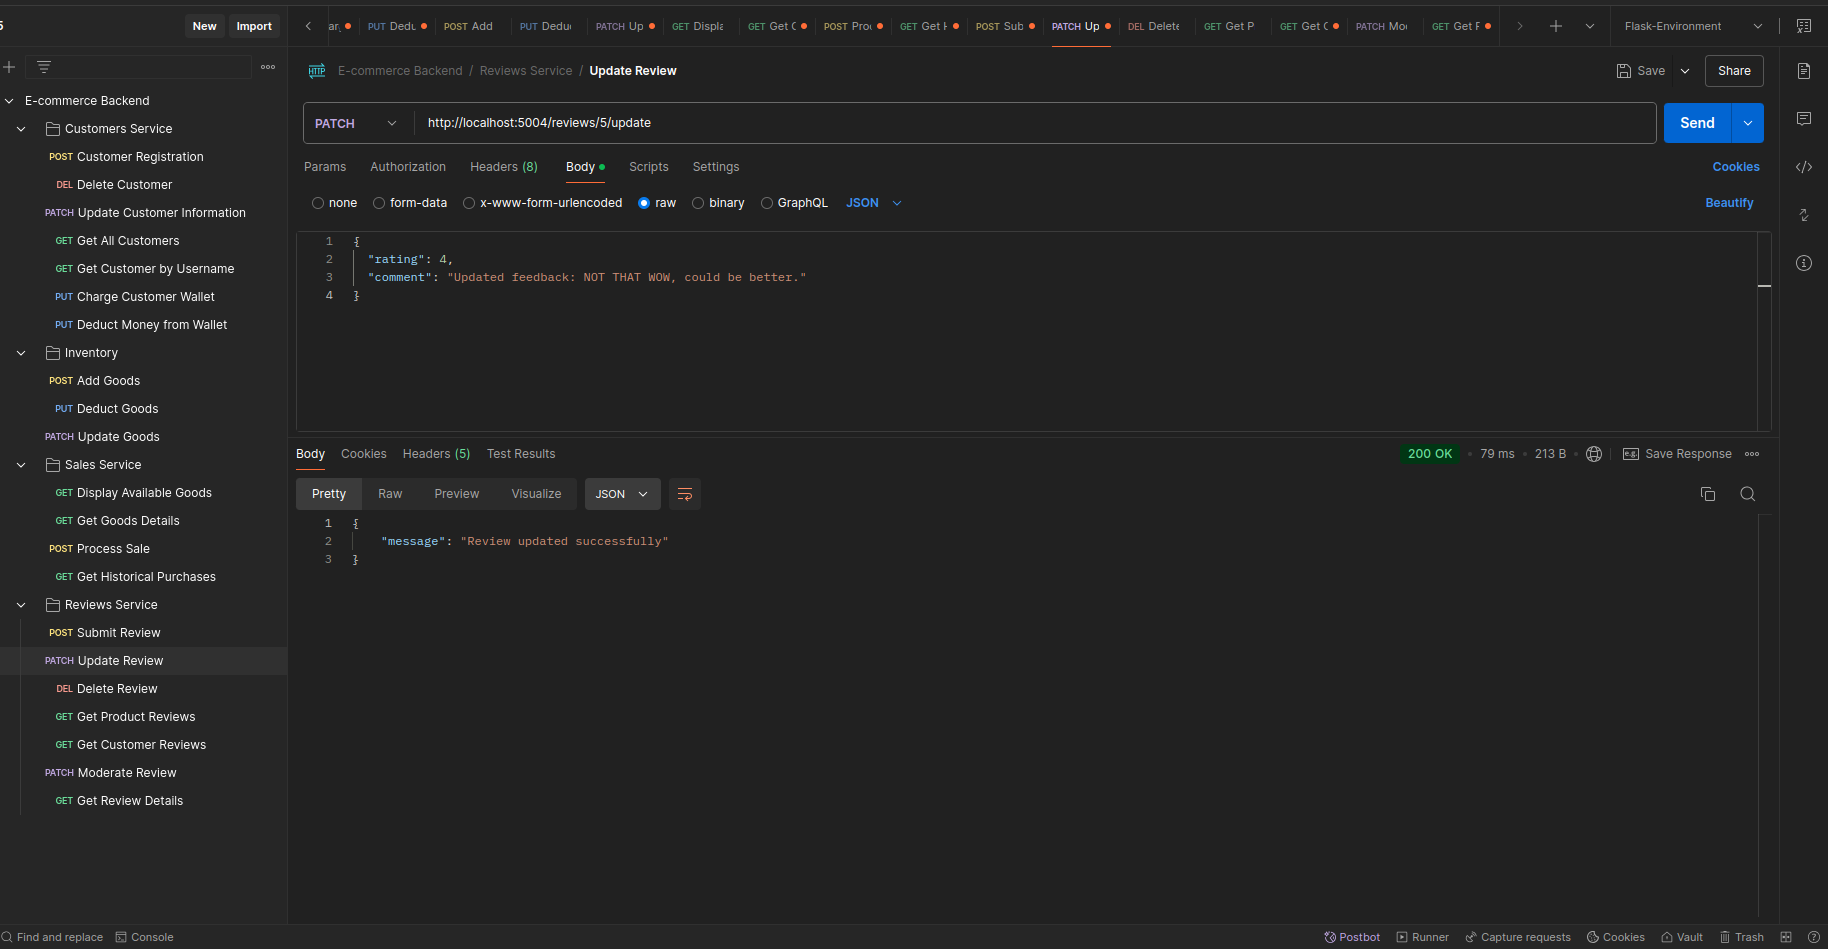
\includegraphics[width=0.6\textwidth]{images/16.png}
  \caption{Update review}
\end{figure}
\begin{figure}[H]
  \centering
  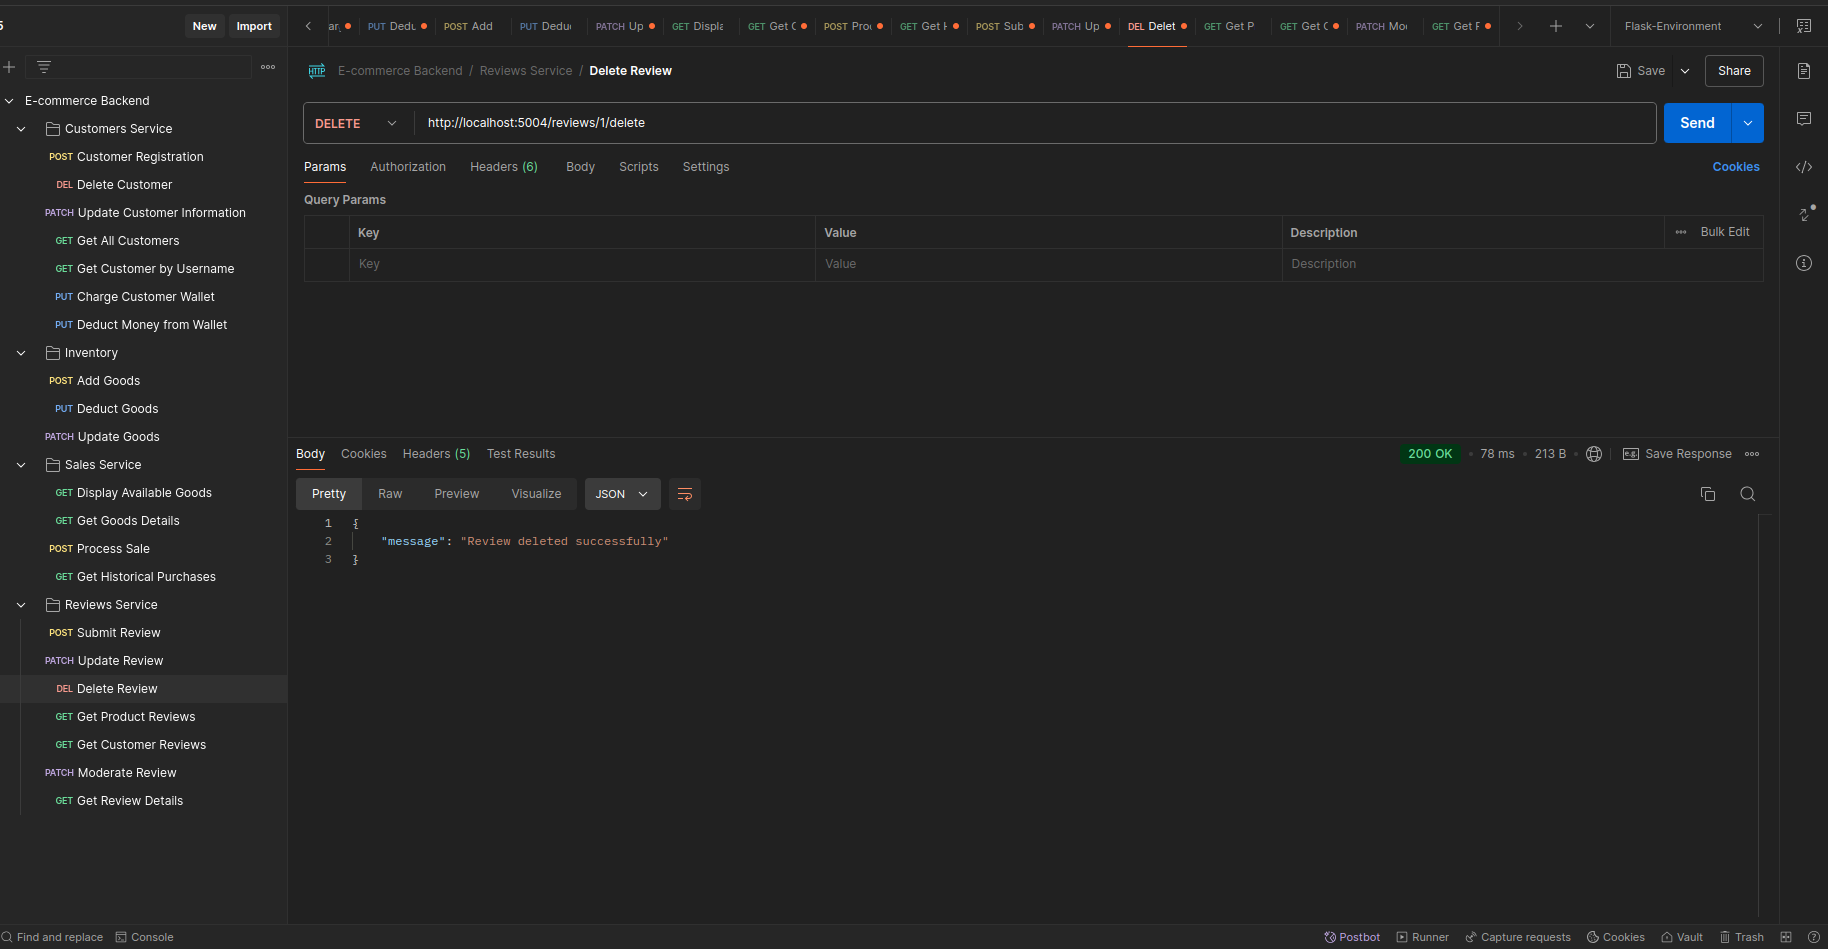
\includegraphics[width=0.6\textwidth]{images/17.png}
  \caption{Delete review}
\end{figure}
\begin{figure}[H]
  \centering
  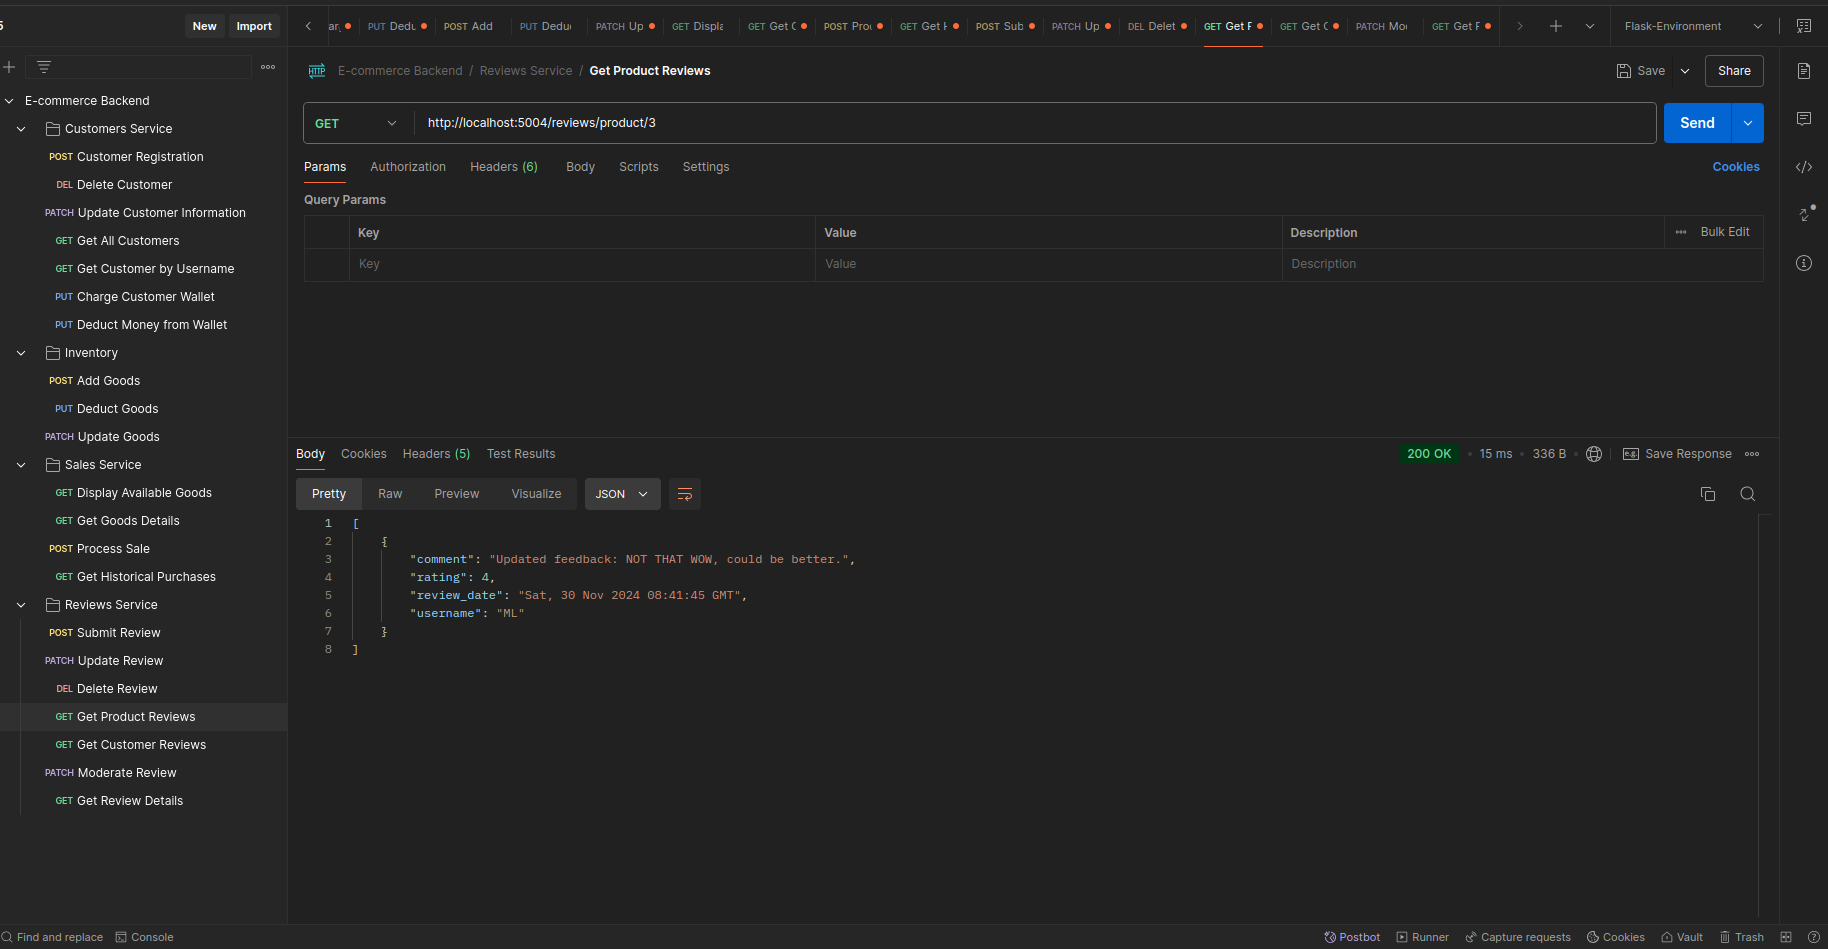
\includegraphics[width=0.6\textwidth]{images/18.png}
  \caption{Get product reviews}
\end{figure}
\begin{figure}[H]
  \centering
  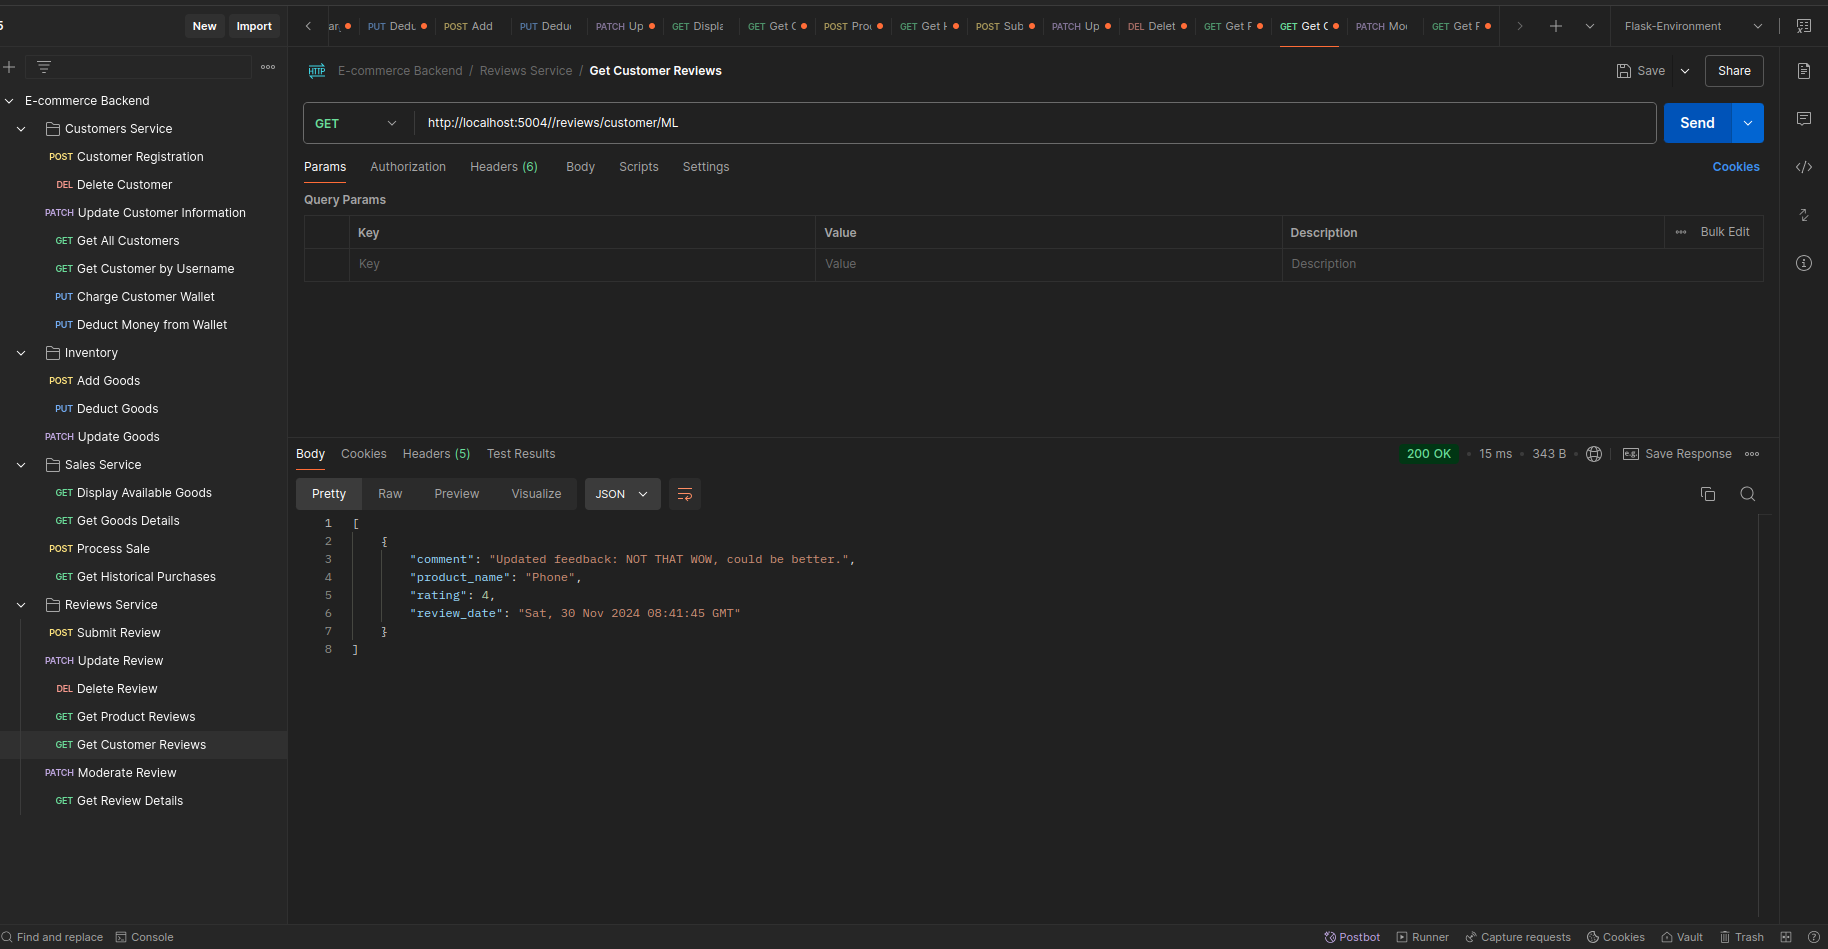
\includegraphics[width=0.6\textwidth]{images/19.png}
  \caption{Get customer reviews}
\end{figure}
\begin{figure}[H]
  \centering
  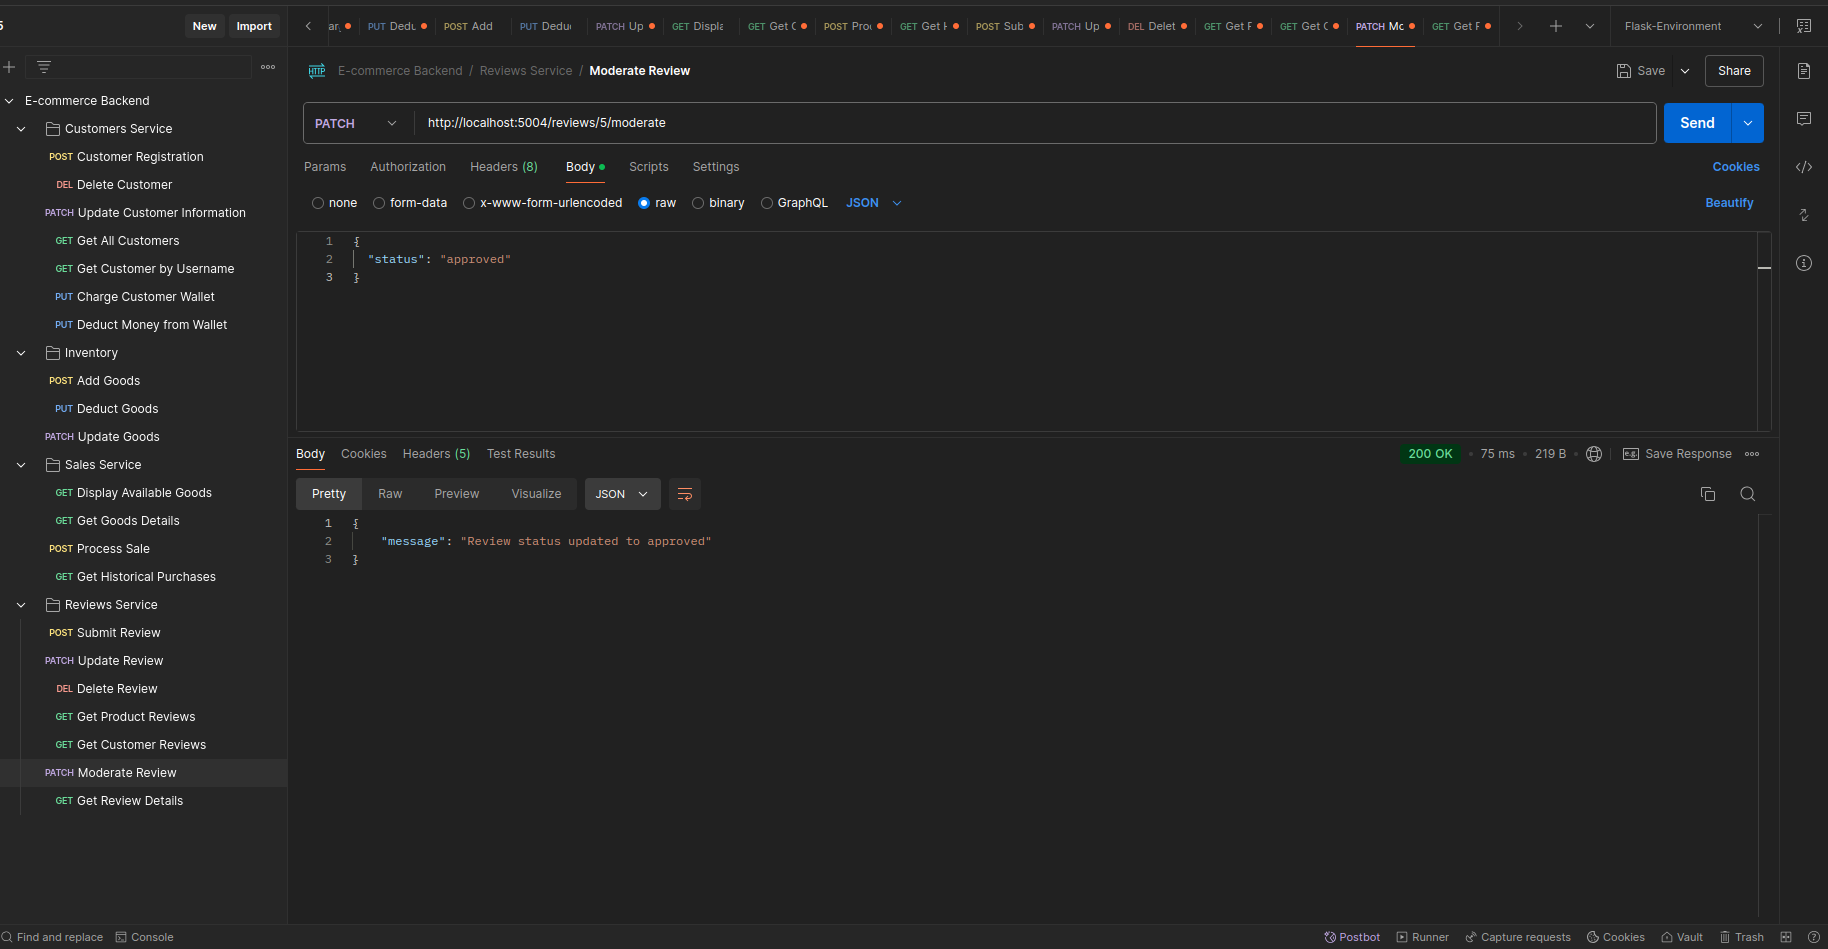
\includegraphics[width=0.6\textwidth]{images/20.png}
  \caption{Moderate review}
\end{figure}
\begin{figure}[H]
  \centering
  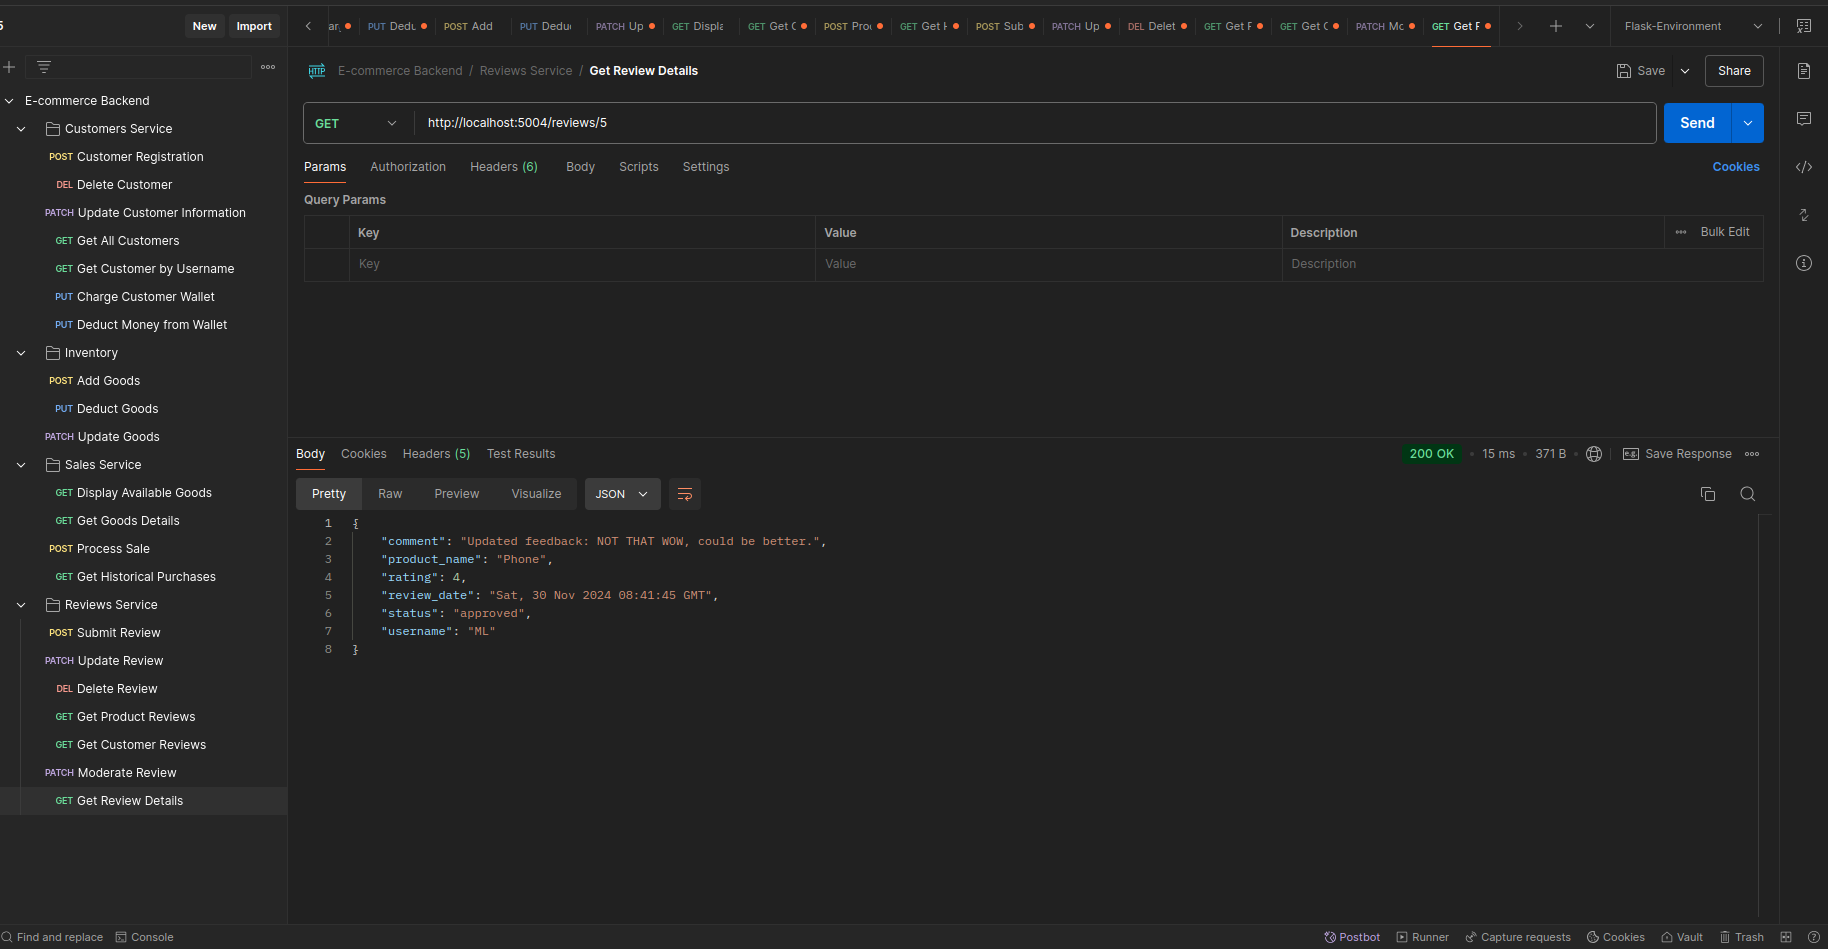
\includegraphics[width=0.6\textwidth]{images/21.png}
  \caption{Get review details}
\end{figure}

\section{Error Handling and Validation}
\subsection{Error Management}
Errors in the system are managed to ensure smooth operations and meaningful responses to clients. The following strategies are implemented:

\begin{enumerate}
    \item \textbf{HTTP Status Codes}
    \begin{itemize}
        \item \textbf{2xx Success Codes:} Indicate successful operations (e.g., \texttt{200 OK}, \texttt{201 Created}).
        \item \textbf{4xx Client Errors:} Inform the client of issues with their request:
        \begin{itemize}
            \item \texttt{400 Bad Request:} Returned for missing or invalid fields in the request payload.
            \item \texttt{404 Not Found:} Returned when the requested resource does not exist.
        \end{itemize}
        \item \textbf{5xx Server Errors:} Catch unexpected errors during processing (e.g., database connection issues).
    \end{itemize}

    \item \textbf{Exception Handling}
    \begin{itemize}
        \item \textbf{Database Exceptions:} Managed using \texttt{try-except} blocks to handle SQL errors and ensure proper rollbacks.
        \item \textbf{Flask-Specific Exceptions:} Use Flask’s built-in error handling to provide user-friendly error messages.
    \end{itemize}

    \item \textbf{Fallback Mechanism:} Unexpected errors return a generic \texttt{500 Internal Server Error} during production, with debug information enabled during development.
\end{enumerate}

\subsection{Validation}
The system includes comprehensive validation to ensure data integrity and appropriate operations. Below are the implemented validations:

\begin{enumerate}
    \item \textbf{Request Payload Validation:}
    \begin{itemize}
        \item Each API validates incoming payloads to ensure required fields are present and properly formatted.
        \item Examples include:
        \begin{itemize}
            \item Customers Service: Ensures username uniqueness and verifies mandatory fields like \texttt{username}, \texttt{password}, and \texttt{age}.
            \item Sales Service: Validates wallet balance and product availability before processing a sale.
            \item Reviews Service: Checks that the \texttt{rating} is between 1 and 5.
        \end{itemize}
    \end{itemize}

    \item \textbf{Database Constraints:}
    \begin{itemize}
        \item Enforced at the schema level:
        \begin{itemize}
            \item Primary Keys prevent duplicate entries.
            \item Foreign Keys ensure relationships between tables are respected (e.g., \texttt{customer\_id} in \texttt{sales\_history} must exist in \texttt{customers} table).
            \item Check Constraints validate numeric ranges (e.g., \texttt{rating} between 1 and 5).
        \end{itemize}
    \end{itemize}

    \item \textbf{Error Response for Missing Resources:}
    \begin{itemize}
        \item APIs return \texttt{404 Not Found} when:
        \begin{itemize}
            \item A customer, product, or review cannot be found.
        \end{itemize}
    \end{itemize}

    \item \textbf{Status Validation in Reviews:}
    \begin{itemize}
        \item Only allows valid statuses (\texttt{approved}, \texttt{flagged}) in the moderation process.
    \end{itemize}

    \item \textbf{Flask-Level Validation:}
    \begin{itemize}
        \item Enforces clean input, such as ensuring numeric IDs (e.g., \texttt{<int:review\_id>}).
    \end{itemize}
\end{enumerate}
\section{User Authentication and Hashing added to the passwords (Point 12)}
\textit{1. Note: So what I did here is that first each customer will have to enter a password when registering, and this password will be hashed using the "bcrypt" library, and then stored in the database. This way the password is secure and not stored in plain text.}\\
\textit{2. Note: I have also added a new field in the customers table called "role" which is defaulted to "user", and only the customers with the role "emp" can delete, submit and update reviews, as requested from \underline{POINT 12}}\\
\subsection{Implementation Details}
\begin{itemize}
    \item \textbf{Input Validation}: The API verifies that all mandatory fields (e.g., full name, username, password, age, address, gender, and marital status) are provided. If any field is missing, an error response is returned to the user.
    \item \textbf{Password Hashing}: To ensure the security of user credentials, the password is hashed before being stored in the database. The \texttt{bcrypt} library is used to generate a secure hashed version of the password using the \texttt{gensalt()} method.
    \item \textbf{Database Interaction}: The API inserts the user’s data into the \texttt{customers} table, including the hashed password and role (defaulted to \texttt{'user'}).
    \item \textbf{Error Handling}: The implementation handles database-specific errors such as duplicate usernames, ensuring appropriate responses are returned to the client.
    \item Now \underline{NOT} any user can delete and submit and update reviews only the ones with the "role" = "emp", they need to provide the correct username and password to be able to do so.
\end{itemize}

\subsection{Postman Testing}
\begin{figure}[H]
  \centering
  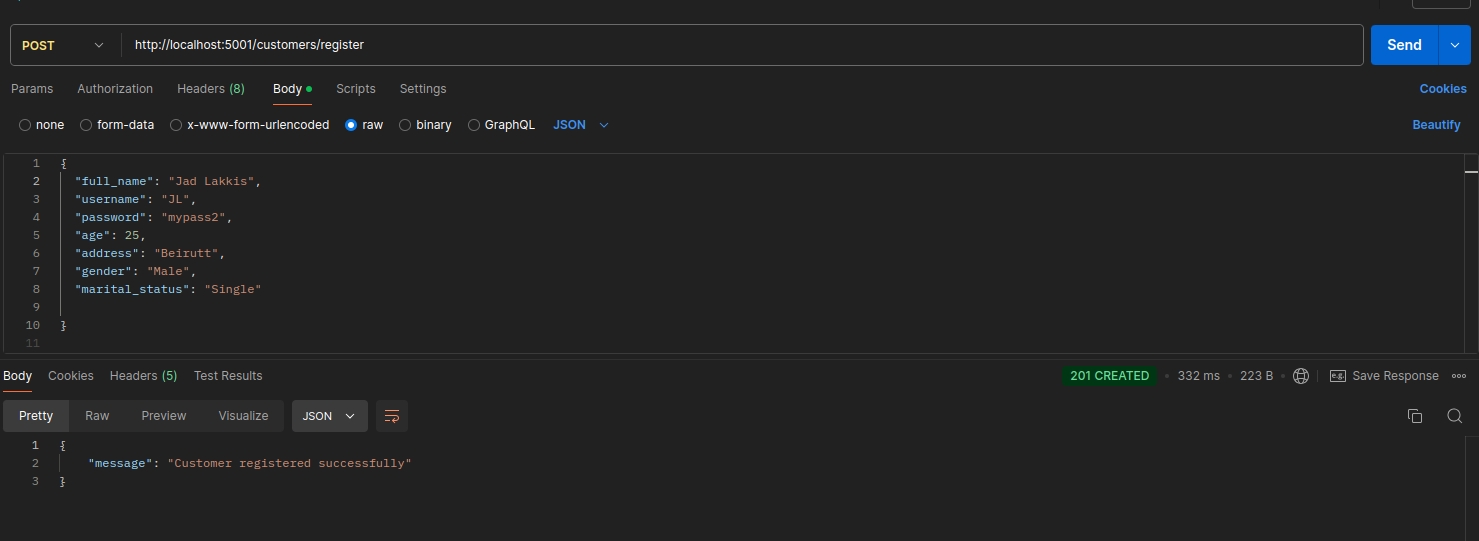
\includegraphics[width=0.6\textwidth]{images/22.png}
  \caption{Registering a new customer role "user"}
\end{figure}
\begin{figure}[H]
  \centering
  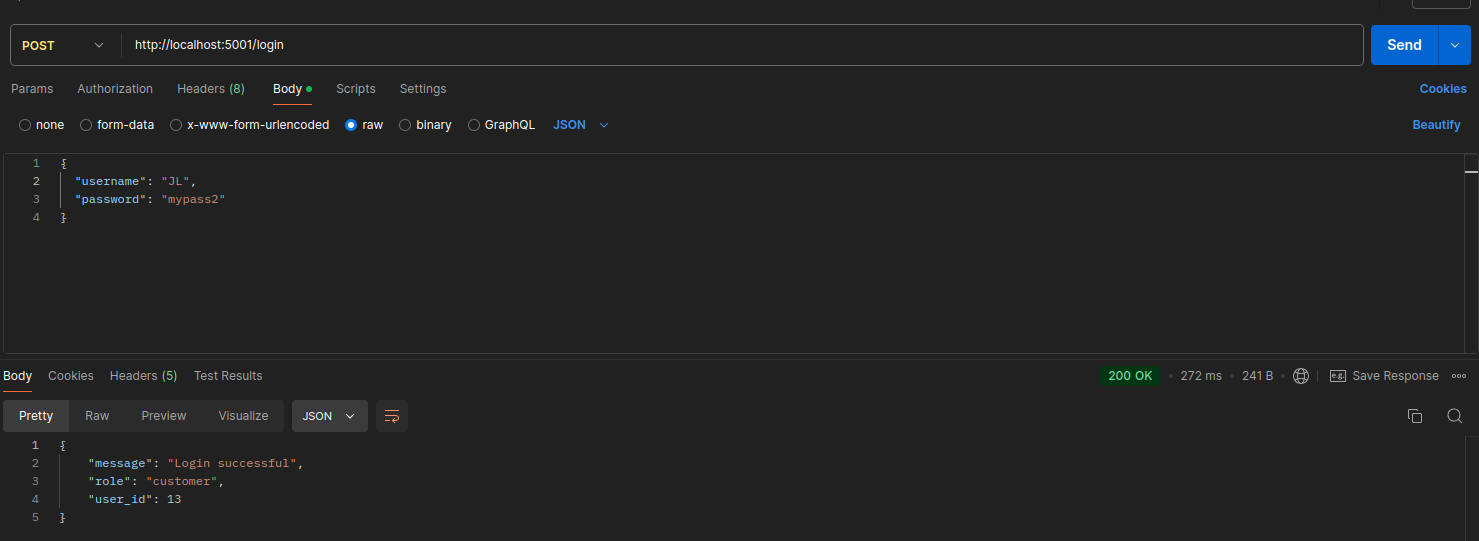
\includegraphics[width=0.6\textwidth]{images/23.png}
  \caption{Login for a customer (this is usrful if we had an interface for the customers to login, but for now it is not used)}
\end{figure}
\begin{figure}[H]
  \centering
  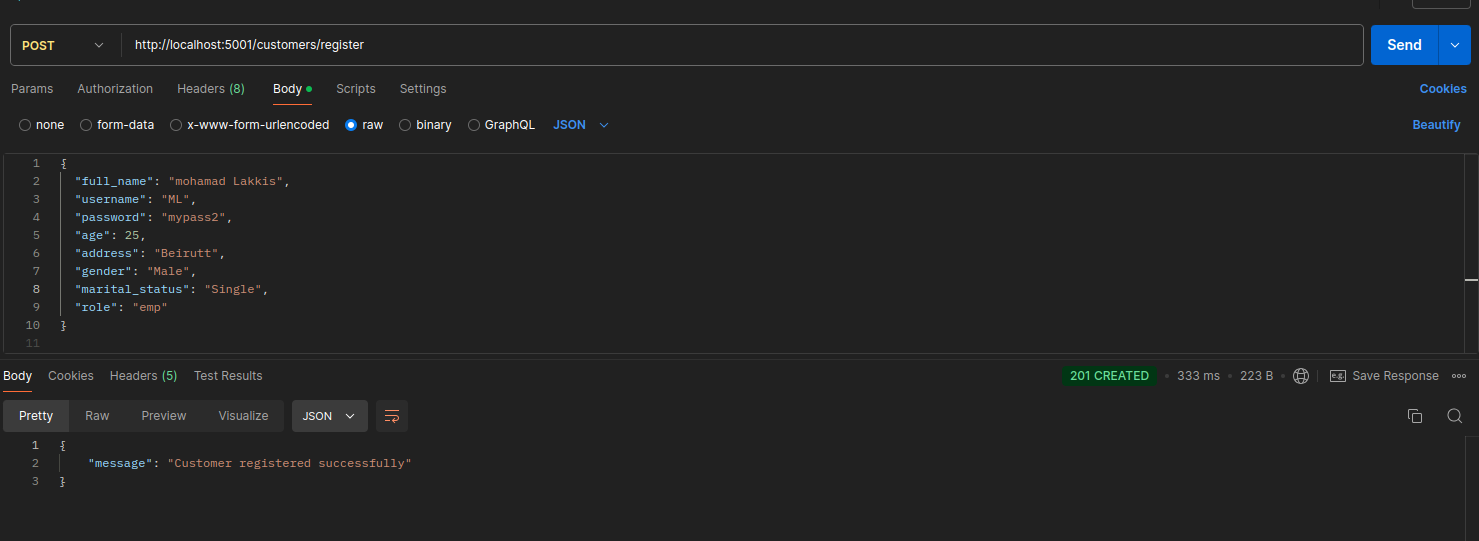
\includegraphics[width=0.6\textwidth]{images/24.png}
  \caption{Registering a new employee}
\end{figure}
\begin{figure}[H]
  \centering
  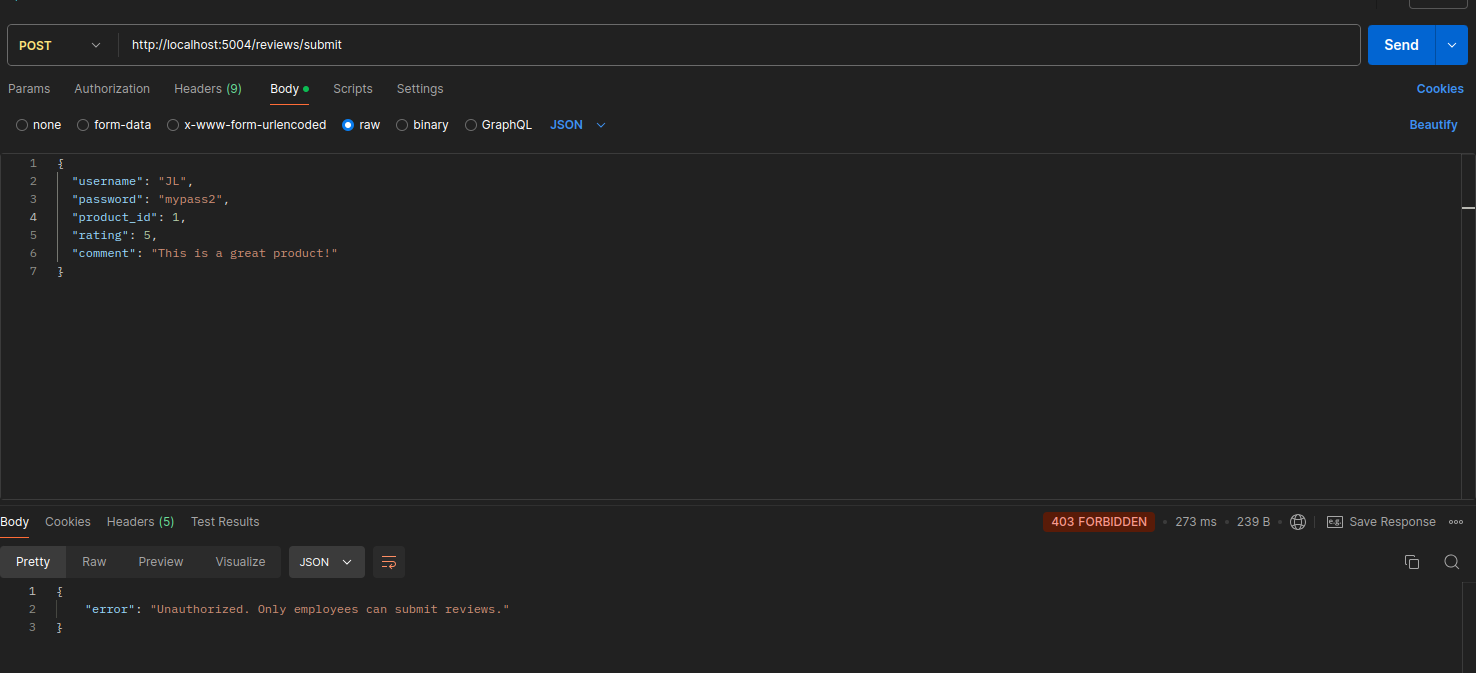
\includegraphics[width=0.6\textwidth]{images/25.png}
  \caption{Attempting to submit a review without the correct role (remember jad is just a customer not an employee, and he won't be able to submit a review) \textbf{NOTE: THAT HERE I COULD HAVE CHANGED THE ROLE TO MAYBE PURCAHSED OR SOMETHING TO ALLOW THE CUSTOMER TO SUBMIT A REVIEW, SINCE IT MAKES SENSE THAT A CUSTOMER CAN SUBMIT A REVIEW, BUT for now I am just following the requirements, and showing that it works, the same is applied if we wanted to do the latter}}
\end{figure}
\begin{figure}[H]
  \centering
  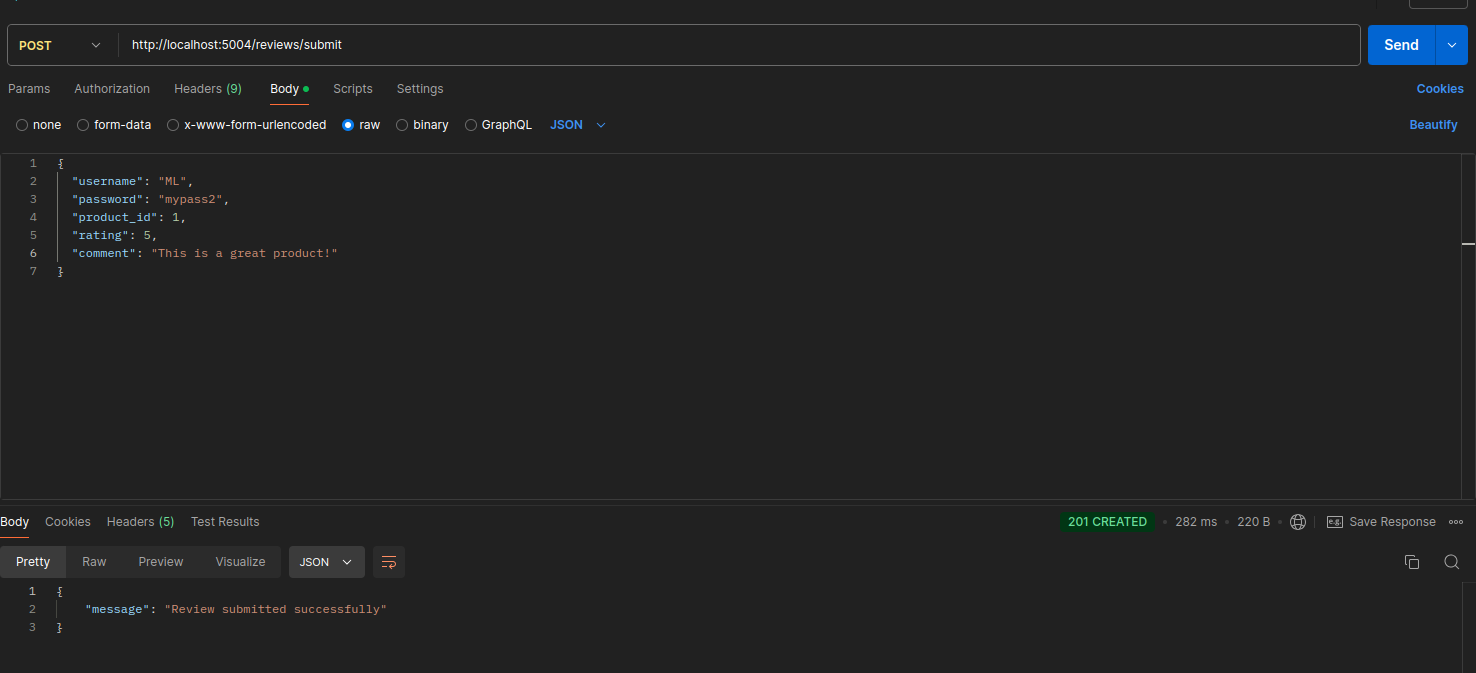
\includegraphics[width=0.6\textwidth]{images/26.png}
  \caption{Submitting a review with the correct role(remember ML is employee and he can submit a review)}
\end{figure}
\begin{figure}[H]
  \centering
  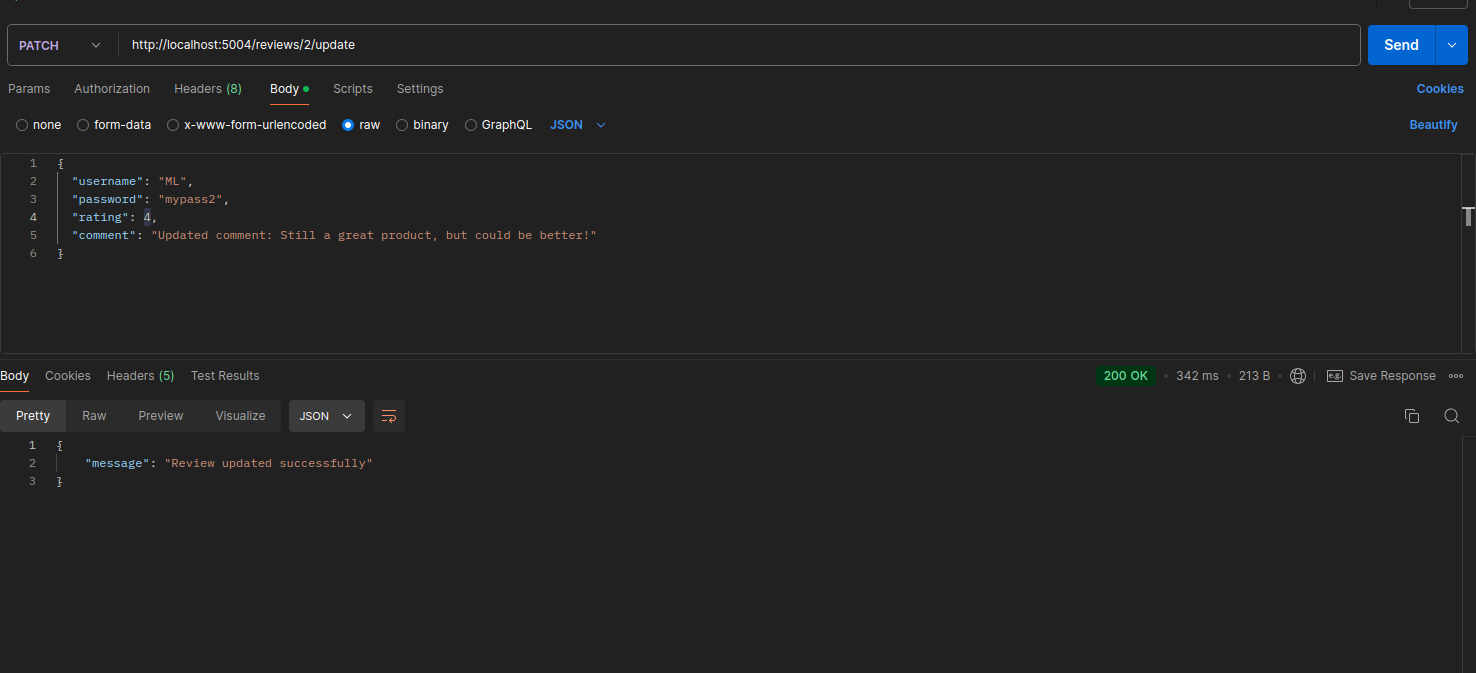
\includegraphics[width=0.6\textwidth]{images/27.png}
  \caption{Updating a review with the correct role}
\end{figure}
\begin{figure}[H]
  \centering
  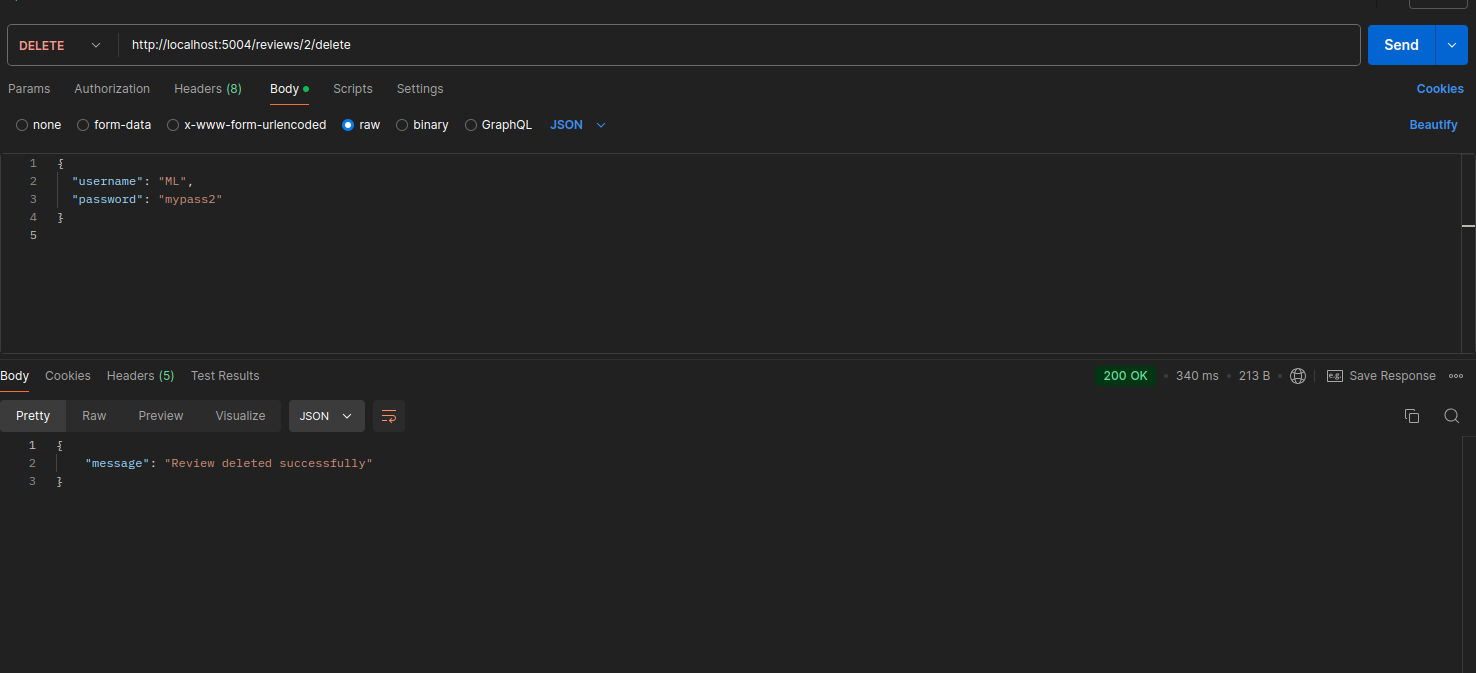
\includegraphics[width=0.6\textwidth]{images/28.png}
  \caption{Deleting a review with the correct role}
\end{figure}
\subsection{Hashing passwords}
\textit{1. Note: remember the passwords we have put for ML and JL, before, now we will take a look at the table to see how they are hashed!}
\begin{figure}[H]
  \centering
  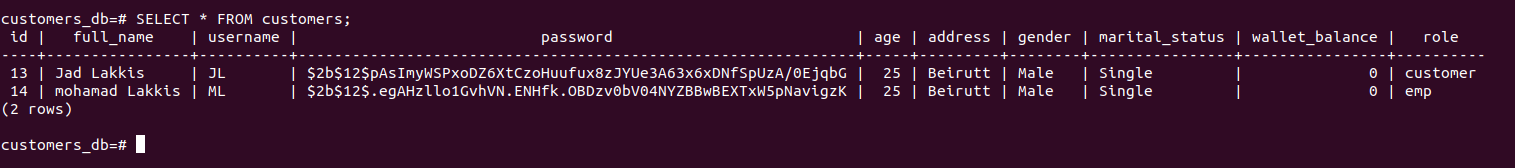
\includegraphics[width=0.6\textwidth]{images/29.png}
  \caption{The passwords are hashed!}
\end{figure}


\section{Validation and Sanitization (point 11)}
\textit{1. Note: I am just showing one part of the code as a proof, in the whole code you can see how the inputs are checcked inside the functions}
\begin{figure}[H]
  \centering
  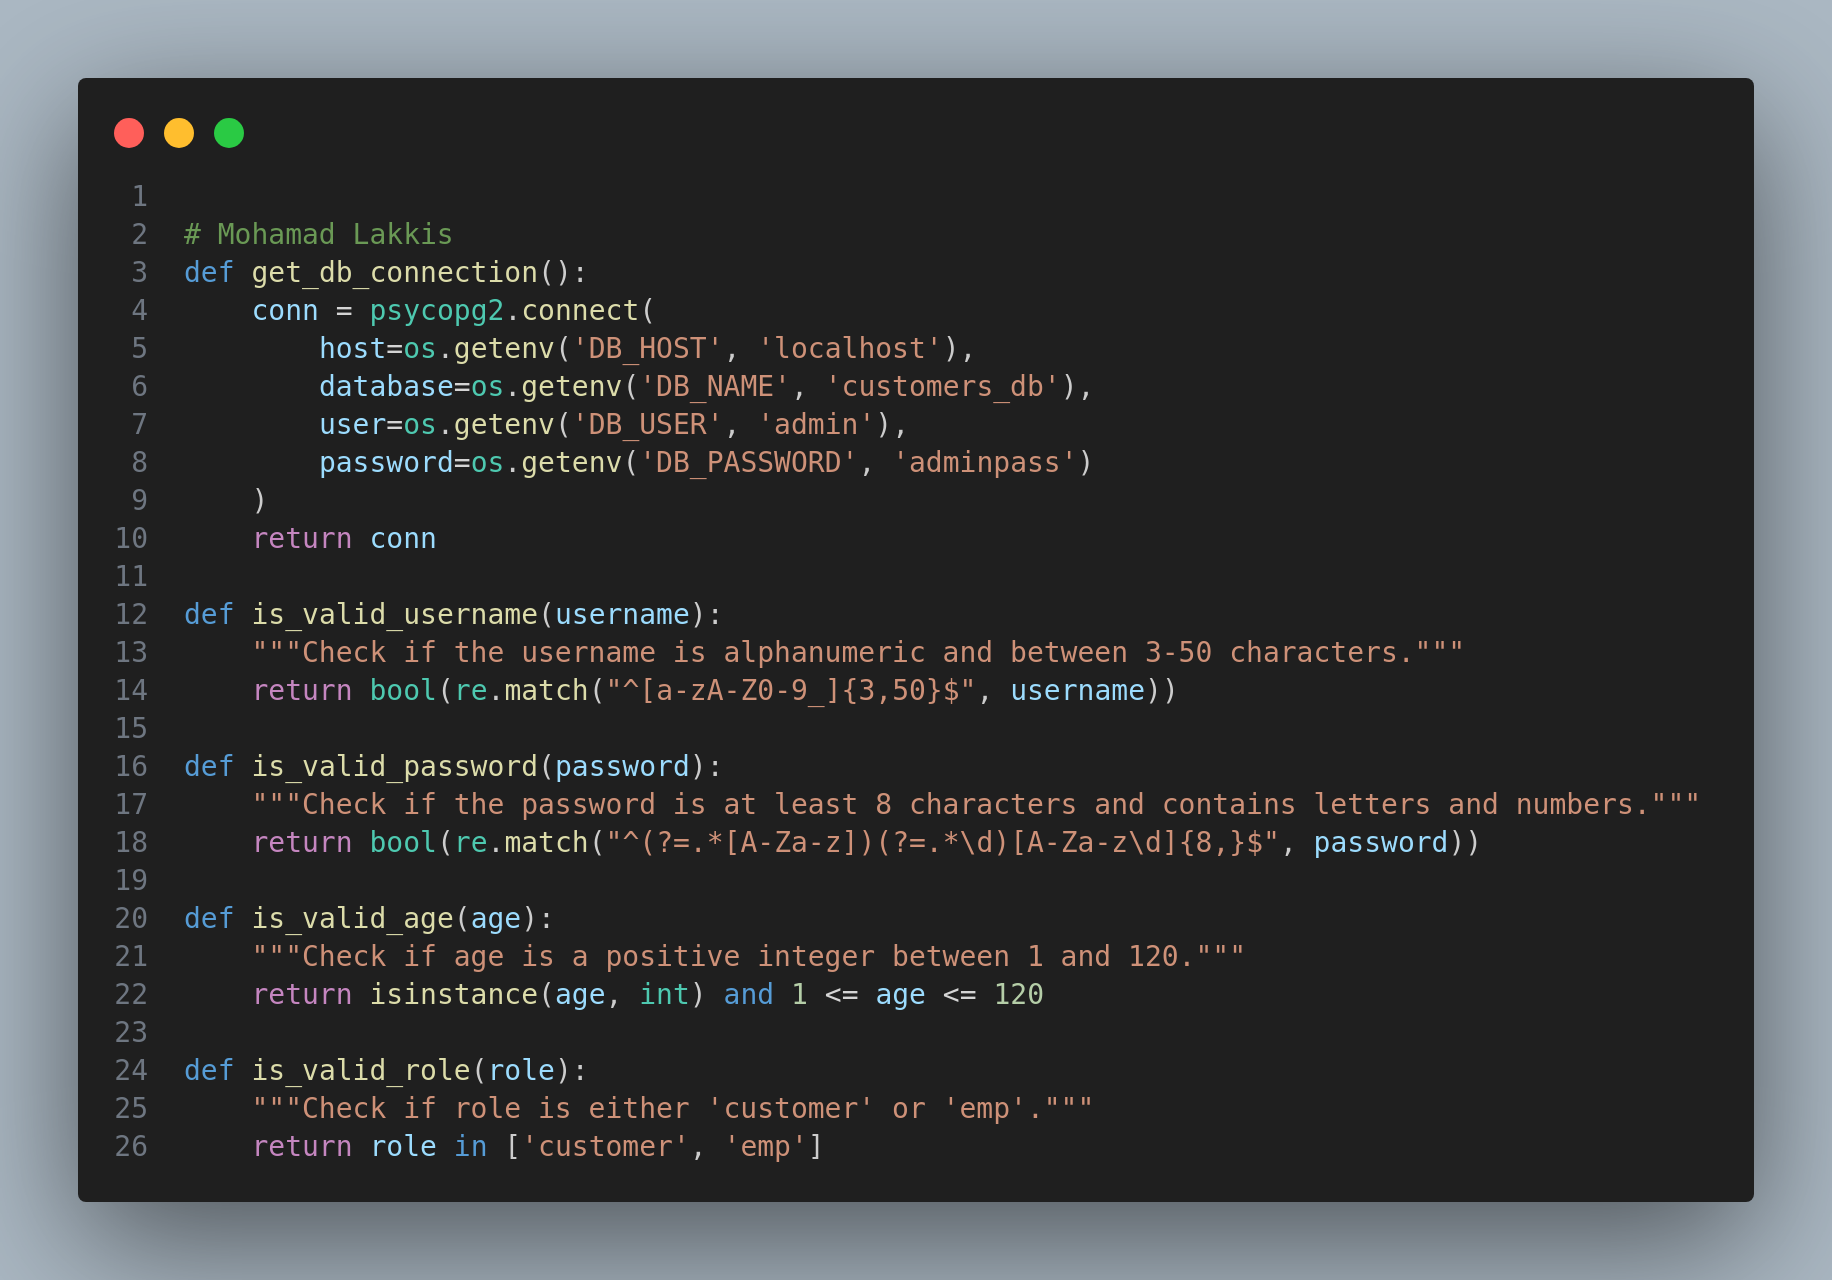
\includegraphics[width=0.6\textwidth]{images/30.png}
  \caption{Validation and Sanitization}
\end{figure}
\begin{figure}[H]
  \centering
  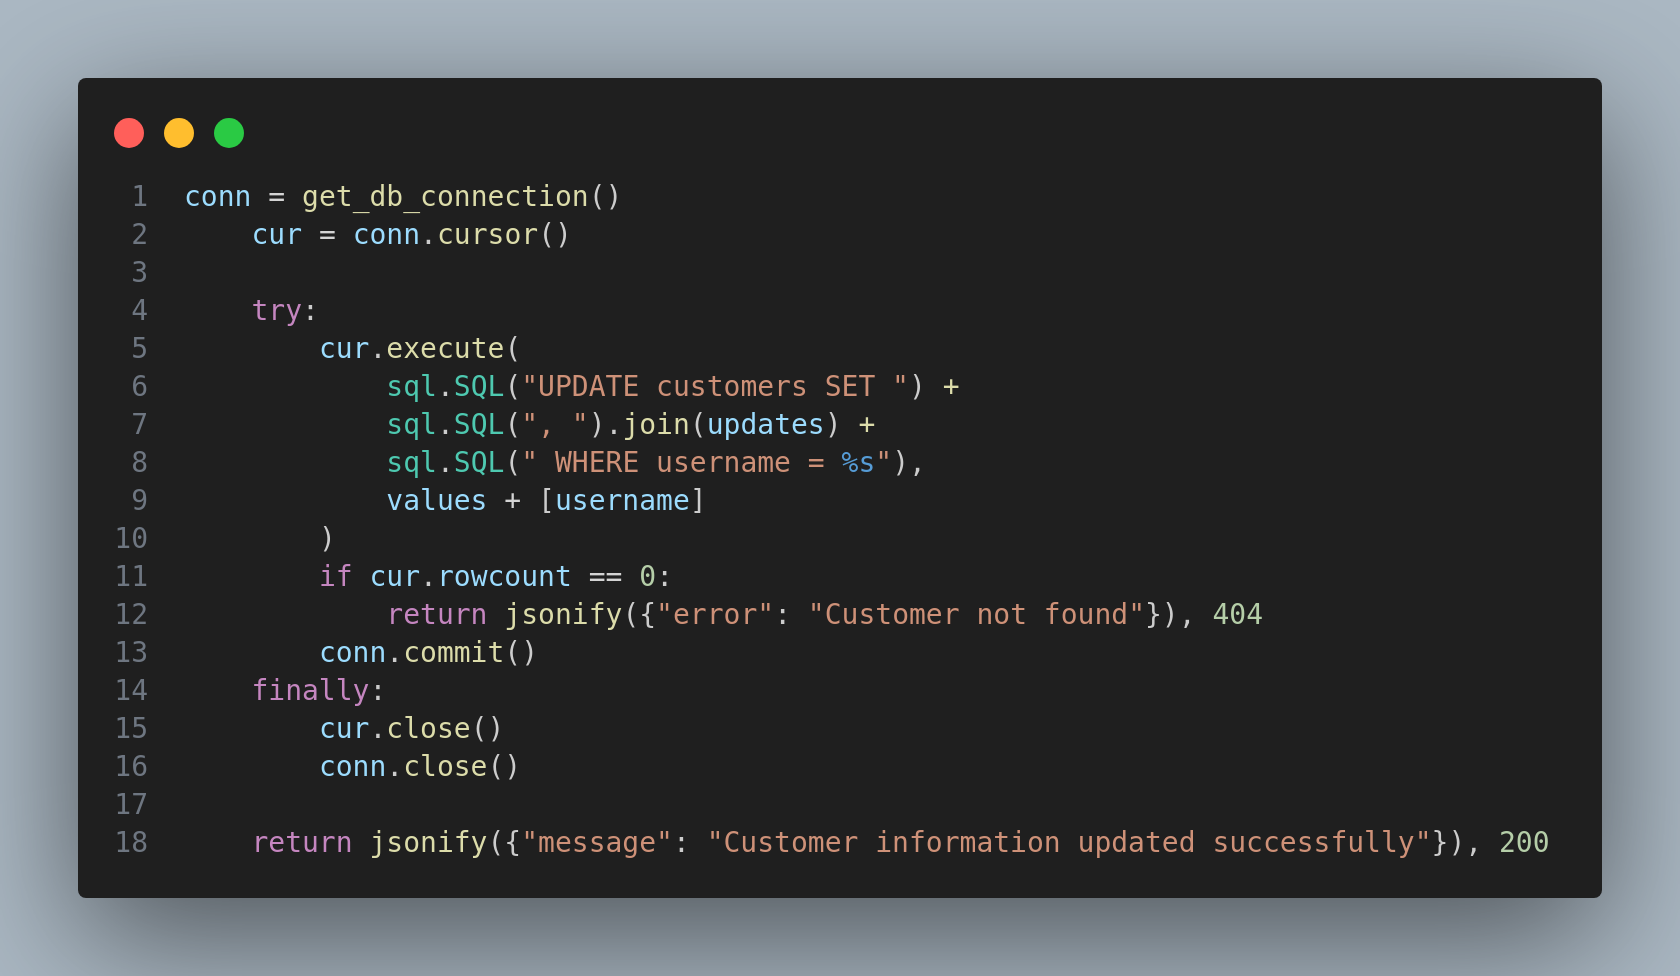
\includegraphics[width=0.6\textwidth]{images/31.png}
  \caption{Validation and Sanitization (another example) there is plenty more in the full codes}
\end{figure}
\section{Moderating (point 13)}
\textit{1. Note: I did similar to authenticator before submitting a review, the user needs to have the role "emp" to able to moderation}
\subsection{Implementation Details}
\begin{figure}[H]
  \centering
  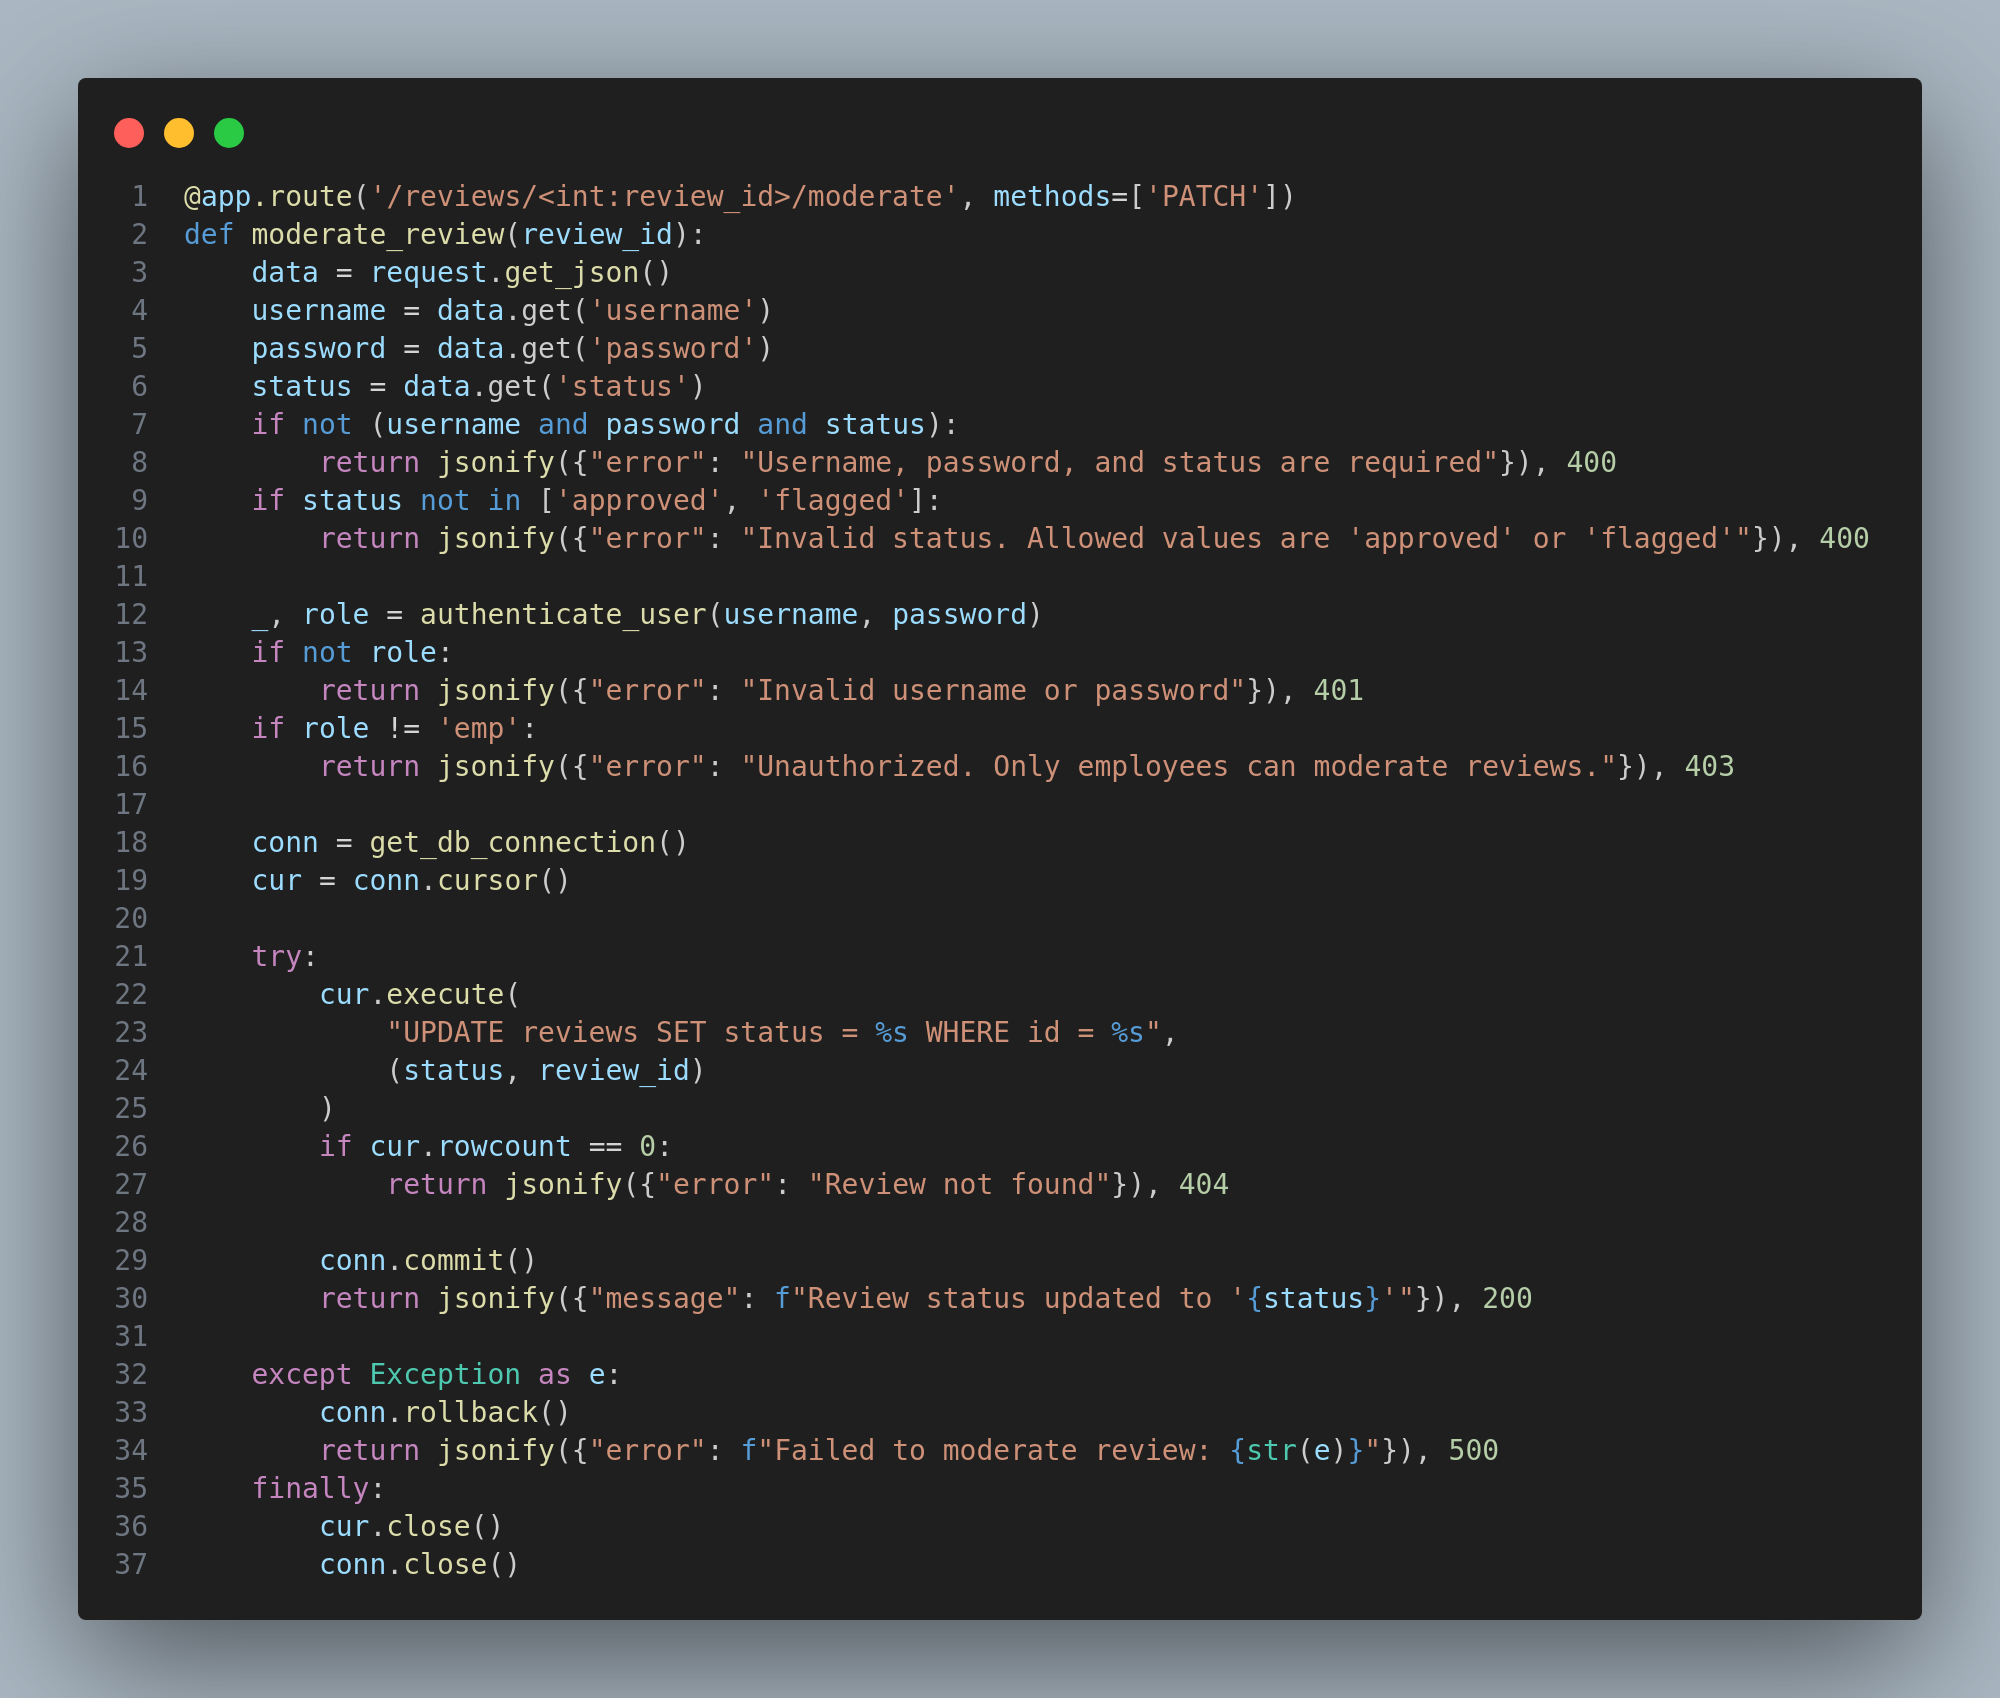
\includegraphics[width=0.6\textwidth]{images/32.png}
  \caption{Moderating a review (the modified code)}
\end{figure}
\subsection{Postman Testing}
\begin{figure}[H]
  \centering
  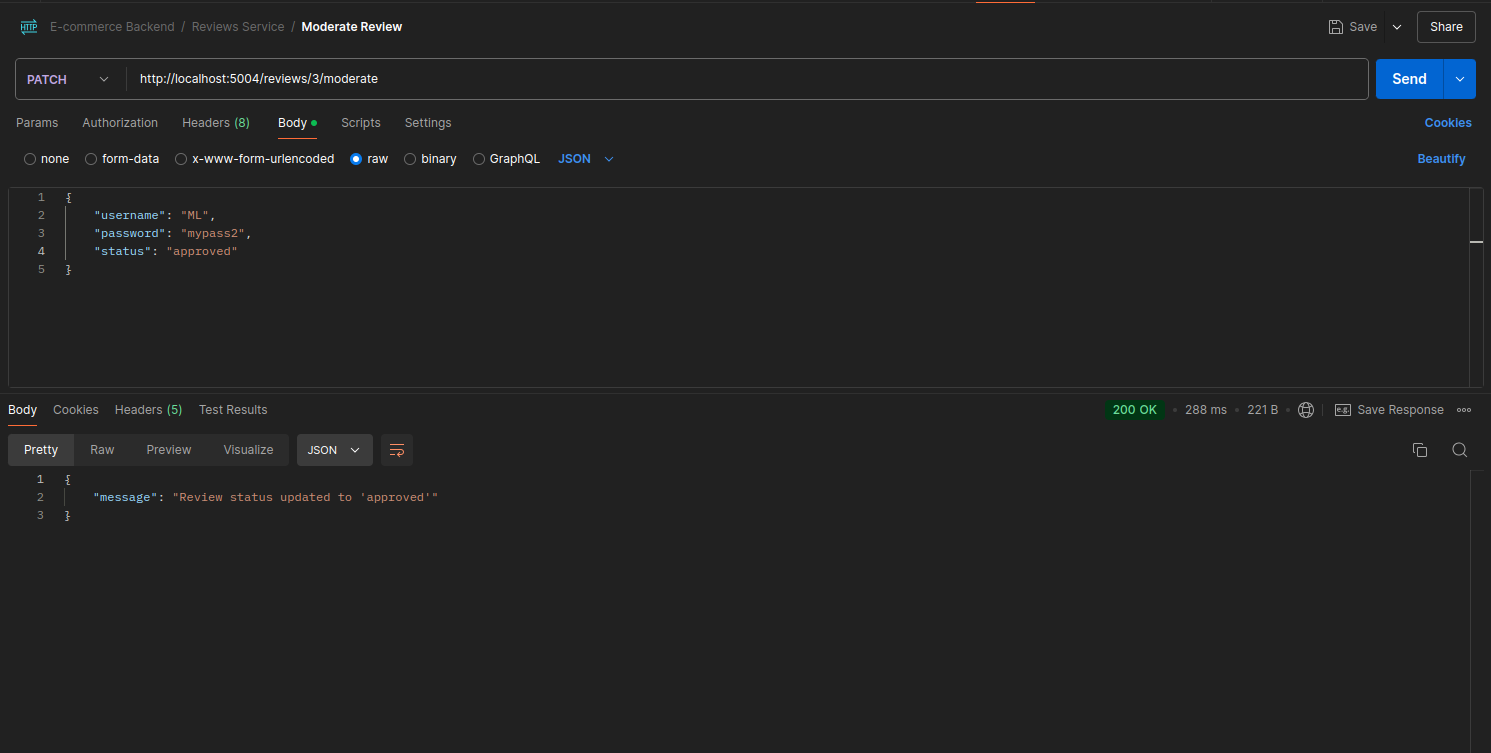
\includegraphics[width=0.6\textwidth]{images/33.png}
  \caption{An example on Postman, using Moderating with a user that has the role "emp"(Remember ML is an employee)}
\end{figure}
\section{Testing (This will cover point 7 from the requirements)}
\textit{1. Note: all of the tests are available in the directory "test" in the submission}
\subsection{Customers API}
\begin{figure}[H]
  \centering
  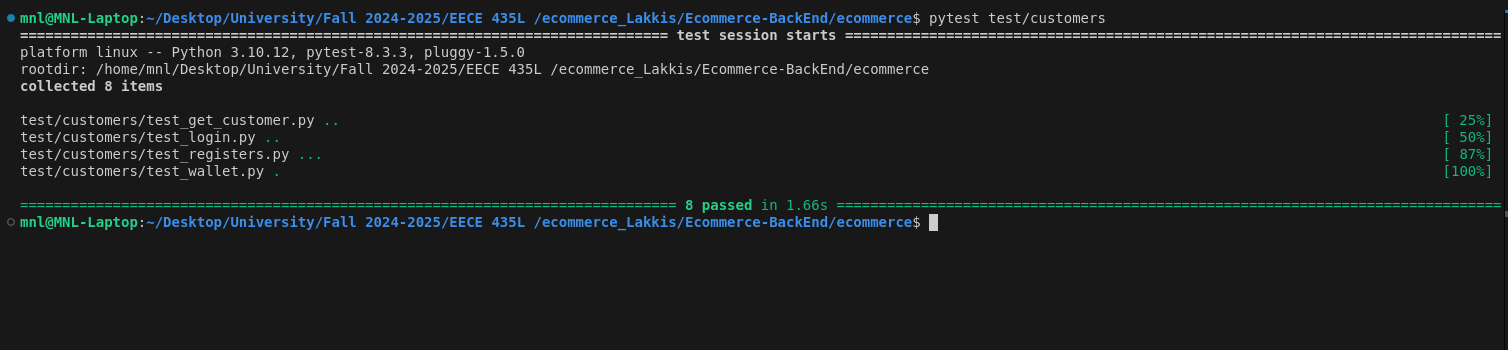
\includegraphics[width=0.6\textwidth]{images/34.png}
  \caption{Testing the Customers API}
\end{figure}
\subsection{Inentory API}
\begin{figure}[H]
  \centering
  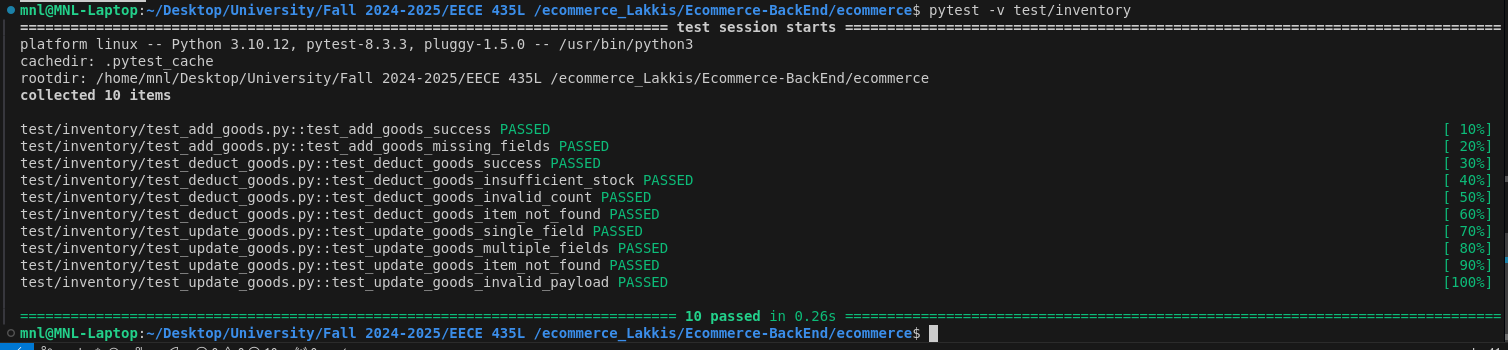
\includegraphics[width=0.6\textwidth]{images/35.png}
  \caption{Testing the Inventory API}
\end{figure}
\subsection{reviews API}
\begin{figure}[H]
  \centering
  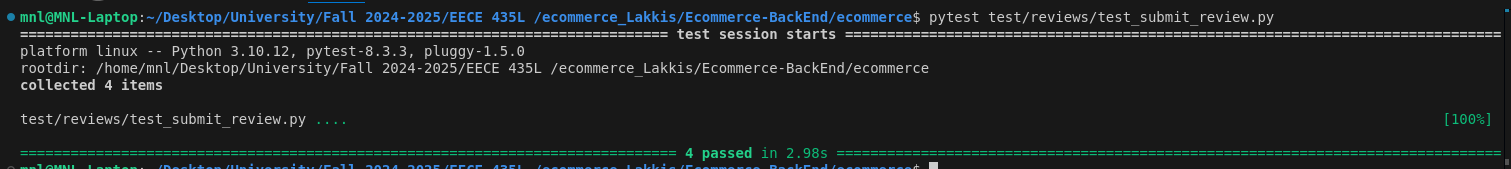
\includegraphics[width=0.6\textwidth]{images/36.png}
  \caption{Testing the Reviews API}
\end{figure}
\subsection{Sales API}
\begin{figure}[H]
  \centering
  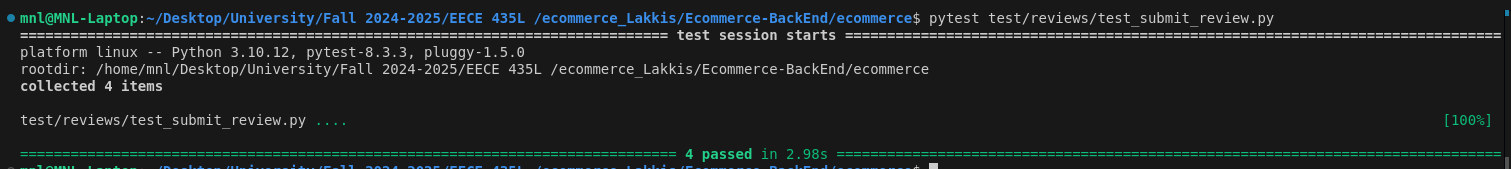
\includegraphics[width=0.6\textwidth]{images/37.png}
  \caption{Testing the Sales API}
\end{figure}
\section{Performance, memory, and code coverage profiling}
\begin{figure}[H]
  \centering
  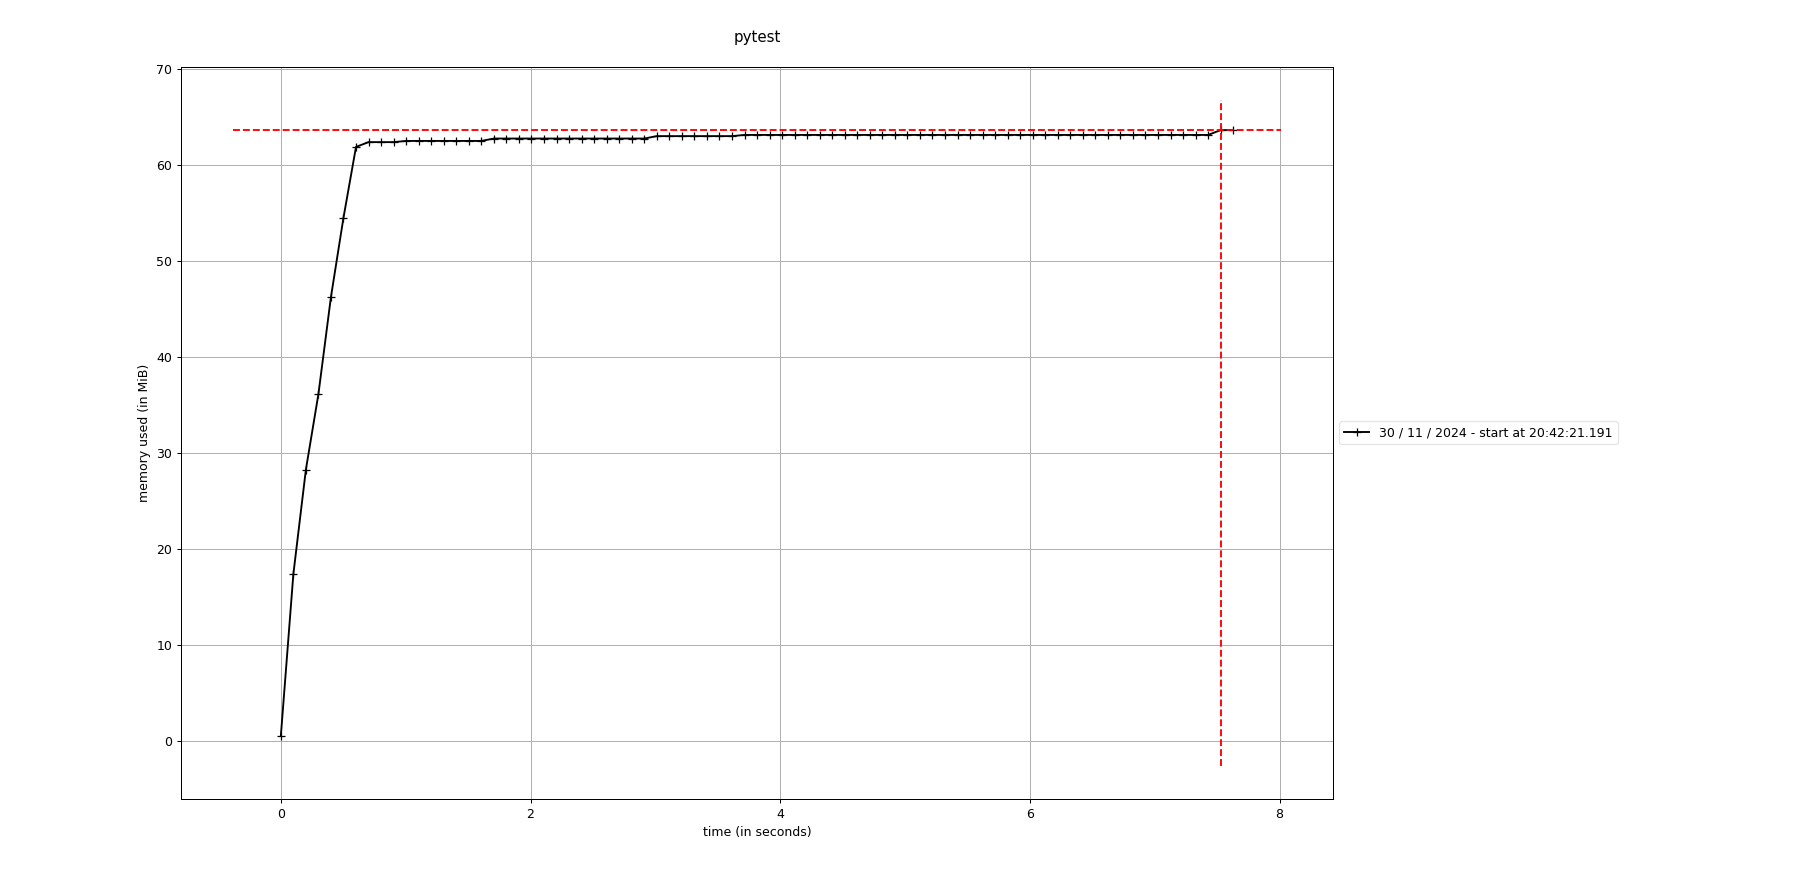
\includegraphics[width=0.6\textwidth]{images/38.png}
  \caption{memory usage graphs}
\end{figure}
\begin{figure}[H]
  \centering
  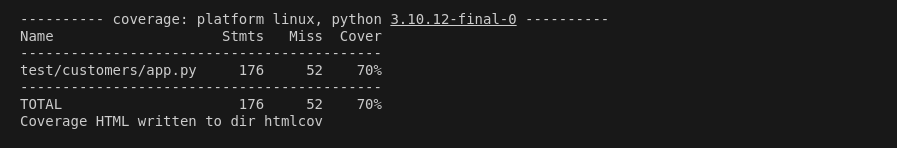
\includegraphics[width=0.6\textwidth]{images/39.png}
  \caption{code coverage}
\end{figure}
\section{Documentation HTML}
\textit{1. Note: Here I provided only a glimpse of the documentation for the full documentation go to "build/html/index.html" in the submission}
\begin{figure}[H]
  \centering
  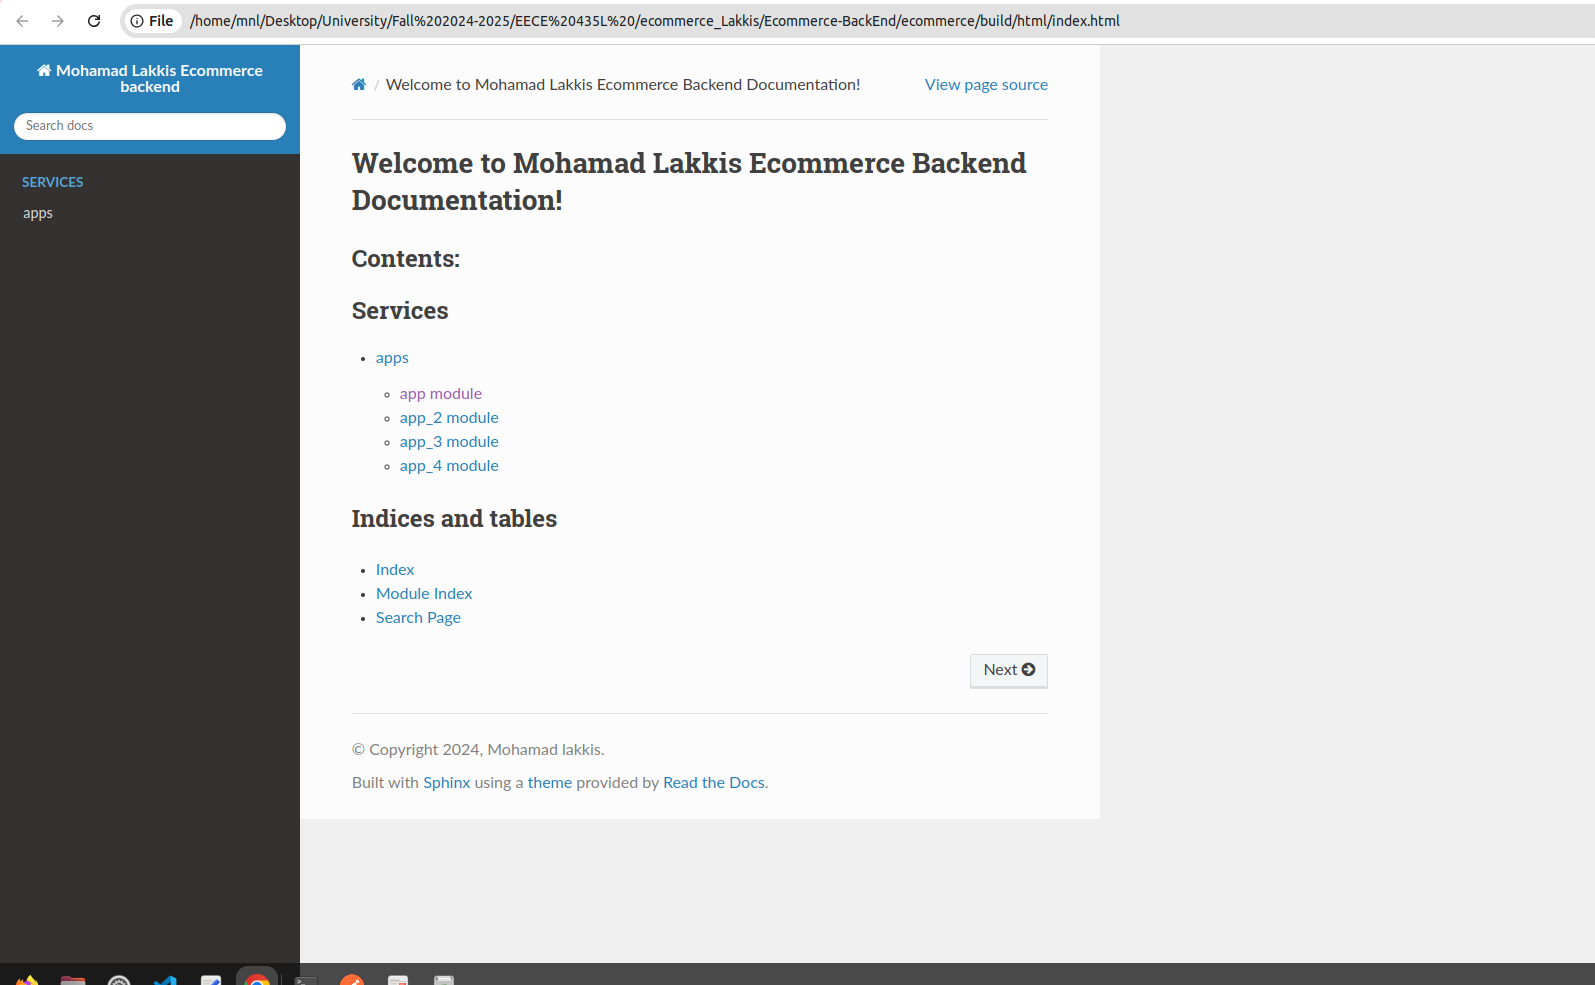
\includegraphics[width=0.9\textwidth]{images/40.png}
  \caption{Documentation HTML (1)}
\end{figure}
\begin{figure}[H]
  \centering
  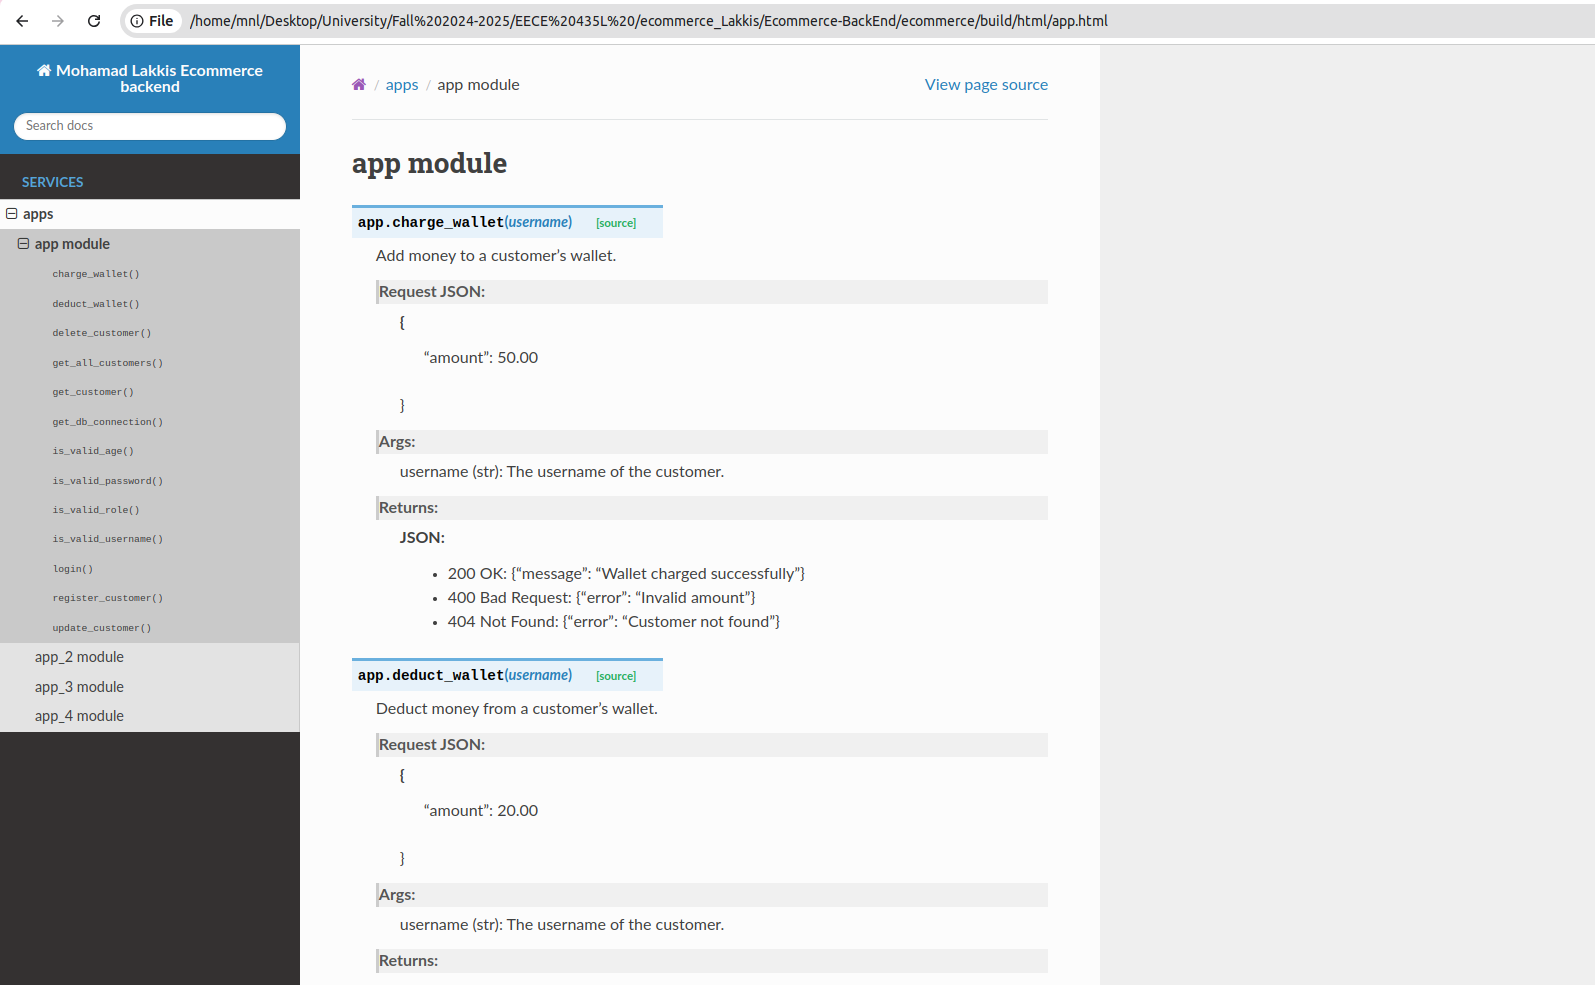
\includegraphics[width=0.9\textwidth]{images/41.png}
  \caption{Documentation HTML (2)}
\end{figure}
\begin{figure}[H]
  \centering
  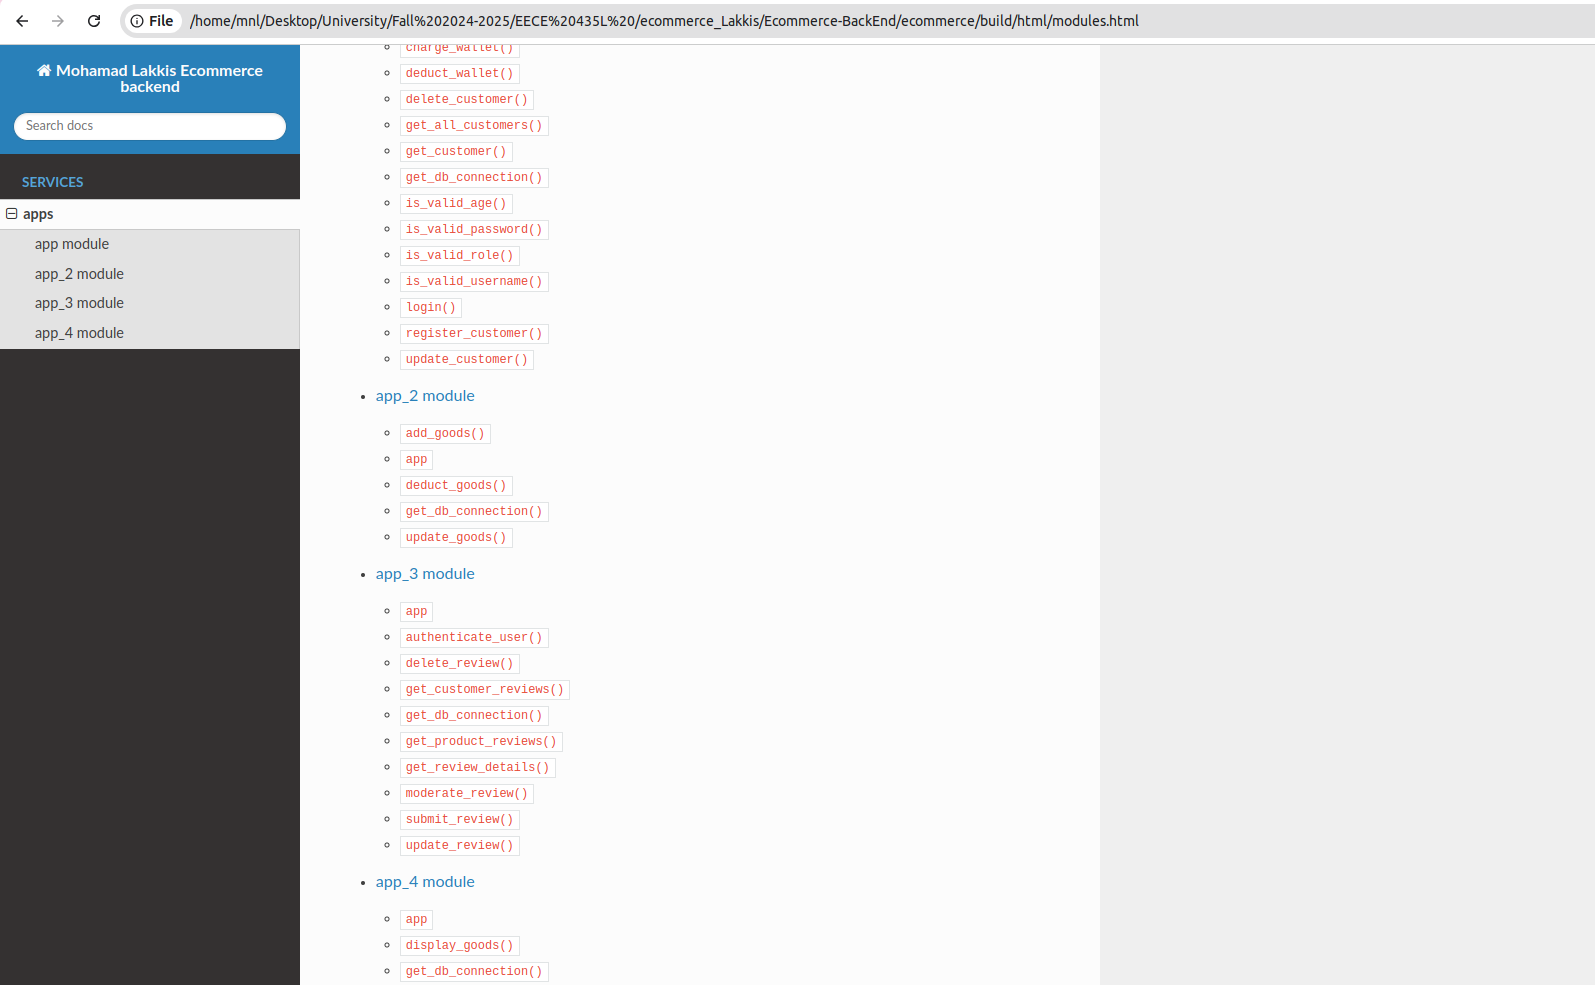
\includegraphics[width=0.9\textwidth]{images/42.png}
  \caption{Documentation HTML (3)}
\end{figure}
\section{Additional Features}

\subsection{Security Measures (point 11)}
\textbf{Security Practices:} To enhance the robustness of the system, several measures have been implemented to prevent common vulnerabilities:

\begin{itemize}
    \item \textbf{SQL Injection Prevention:}
    \begin{itemize}
        \item Prepared Statements and Parameterized Queries are used for all database interactions, ensuring user inputs are never directly concatenated into SQL queries, thereby preventing SQL injection attacks.
        \item Example:
        \begin{verbatim}
        query = "SELECT * FROM customers WHERE username = %s"
        cursor.execute(query, (username,))
        \end{verbatim}
    \end{itemize}

    \item \textbf{Input Validation and Sanitization:}
    \begin{itemize}
        \item All inputs are rigorously validated and sanitized at the API layer. 
        \item For instance, username fields are restricted to alphanumeric characters, and passwords are checked for length and complexity.
    \end{itemize}

    \item \textbf{Authentication and Authorization:}
    \begin{itemize}
        \item The \texttt{bcrypt} library is used to securely hash passwords. Only hashed passwords are stored in the database.
        \item Role-based access control (RBAC) is enforced. For example:
        \begin{itemize}
            \item Only users with the role \texttt{emp} can moderate reviews.
            \item Customers can only access and modify their own data.
        \end{itemize}
    \end{itemize}

    \item \textbf{Secure Communication:}
    \begin{itemize}
        \item The APIs are designed to run behind HTTPS. For local development, Flask’s \texttt{ssl\_context} is used to enable TLS.
    \end{itemize}

    \item \textbf{Error Message Minimization:}
    \begin{itemize}
        \item Detailed error messages that could reveal internal logic or structure are avoided in production. Generic error messages are displayed to users, while detailed logs are stored for developers.
    \end{itemize}
\end{itemize}

\subsection{Advanced Development Practices(point 7)}

\textbf{Custom Exception Handling:} A standardized framework for exception handling has been implemented to ensure clear and consistent error messaging across all services.

\begin{itemize}
    \item \textbf{Centralized Error Handler:}
    \begin{itemize}
        \item Each service includes a centralized error handler that captures exceptions and returns structured JSON responses with appropriate HTTP status codes.
        \item Example:
        \begin{verbatim}
        @app.errorhandler(Exception)
        def handle_exception(e):
            return {
                "error": str(e),
                "message": "An error occurred. Please try again later."
            }, 500
        \end{verbatim}
    \end{itemize}

    \item \textbf{Service-Specific Exceptions:}
    \begin{itemize}
        \item Custom exceptions have been defined for scenarios like \texttt{UserNotFoundException} or \texttt{InsufficientFundsException}.
        \item These exceptions are caught at the application layer and return user-friendly error messages.
    \end{itemize}
\end{itemize}

\textbf{Versioning APIs:} To maintain backward compatibility and support evolving requirements, API versioning has been implemented.

\begin{itemize}
    \item \textbf{URI-Based Versioning:}
    \begin{itemize}
        \item Each service exposes APIs under versioned paths (e.g., \texttt{/v1/customers}, \texttt{/v1/inventory}).
        \item As APIs evolve, new versions (e.g., \texttt{/v2/customers}) can be introduced without breaking existing clients.
    \end{itemize}

    \item \textbf{Implementation Details:}
    \begin{itemize}
        \item API routers are configured to direct requests to the appropriate version.
        \item Example:
        \begin{verbatim}
        from flask import Blueprint
        v1 = Blueprint('v1', __name__, url_prefix='/v1')
        v2 = Blueprint('v2', __name__, url_prefix='/v2')

        # Register blueprints
        app.register_blueprint(v1)
        app.register_blueprint(v2)
        \end{verbatim}
    \end{itemize}
\end{itemize}

\section{Conclusion}
for the rest please see the code :) \\ 
very nice journey and thank you for your effort and time, in correcting it and reading it, I hope you have a great day!\\
\end{document}
